%%
%% This is file `sigconf.tex',
%% generated with the docstrip utility.
%%
%% The original source files were:
%%
%% samples.dtx  (with options: `all,proceedings,sigconf')
%% 
%% IMPORTANT NOTICE:
%% 
%% For the copyright see the source file.
%% 
%% Any modified versions of this file must be renamed
%% with new filenames distinct from sigconf.tex.
%% 
%% For distribution of the original source see the terms
%% for copying and modification in the file samples.dtx.
%% 
%% This generated file may be distributed as long as the
%% original source files, as listed above, are part of the
%% same distribution. (The sources need not necessarily be
%% in the same archive or directory.)
%%
%%
%% Commands for TeXCount
%TC:macro \cite [option:text,text]
%TC:macro \citep [option:text,text]
%TC:macro \citet [option:text,text]
%TC:envir table 0 1
%TC:envir table* 0 1
%TC:envir tabular [ignore] word
%TC:envir displaymath 0 word
%TC:envir math 0 word
%TC:envir comment 0 0
%%
%% The first command in your LaTeX source must be the \documentclass
%% command.
%%
%% For submission and review of your manuscript please change the
%% command to \documentclass[manuscript, screen, review]{acmart}.
%%
%% When submitting camera ready or to TAPS, please change the command
%% to \documentclass[sigconf]{acmart} or whichever template is required
%% for your publication.
%%
%%

% \documentclass[sigconf]{acmart}
\documentclass[sigconf, anonymous, review]{acmart}

% \settopmatter{printacmref=false}

% other packages needed in this paper
\usepackage{subcaption}
\usepackage{amsthm}
\usepackage{multirow}
\newtheorem{definition}{Definition}

%%
%% \BibTeX command to typeset BibTeX logo in the docs
\AtBeginDocument{%
  \providecommand\BibTeX{{%
    Bib\TeX}}}

%% Rights management information.  This information is sent to you
%% when you complete the rights form.  These commands have SAMPLE
%% values in them; it is your responsibility as an author to replace
%% the commands and values with those provided to you when you
%% complete the rights form.
% \setcopyright{acmlicensed}
% \copyrightyear{2018}
% \acmYear{2018}
% \acmDOI{XXXXXXX.XXXXXXX}
%% These commands are for a PROCEEDINGS abstract or paper.
% \acmConference[Conference acronym 'XX]{Make sure to enter the correct
%   conference title from your rights confirmation email}{June 03--05,
%   2018}{Woodstock, NY}
%%
%%  Uncomment \acmBooktitle if the title of the proceedings is different
%%  from ``Proceedings of ...''!
%%
%%\acmBooktitle{Woodstock '18: ACM Symposium on Neural Gaze Detection,
%%  June 03--05, 2018, Woodstock, NY}
% \acmISBN{978-1-4503-XXXX-X/2018/06}


%%
%% Submission ID.
%% Use this when submitting an article to a sponsored event. You'll
%% receive a unique submission ID from the organizers
%% of the event, and this ID should be used as the parameter to this command.
%%\acmSubmissionID{123-A56-BU3}

%%
%% For managing citations, it is recommended to use bibliography
%% files in BibTeX format.
%%
%% You can then either use BibTeX with the ACM-Reference-Format style,
%% or BibLaTeX with the acmnumeric or acmauthoryear sytles, that include
%% support for advanced citation of software artefact from the
%% biblatex-software package, also separately available on CTAN.
%%
%% Look at the sample-*-biblatex.tex files for templates showcasing
%% the biblatex styles.
%%
%%
%% The majority of ACM publications use numbered citations and
%% references.  The command \citestyle{authoryear} switches to the
%% "author year" style.
%%
%% If you are preparing content for an event
%% sponsored by ACM SIGGRAPH, you must use the "author year" style of
%% citations and references.
%% Uncommenting
%% the next command will enable that style.
%%\citestyle{acmauthoryear}


%%
%% end of the preamble, start of the body of the document source.
\begin{document}

%%
%% The "title" command has an optional parameter,
%% allowing the author to define a "short title" to be used in page headers.
\title{TRINA: Robust Graph Learning for Node Classification Against Trilateral Noise}

%%
%% The "author" command and its associated commands are used to define
%% the authors and their affiliations.
%% Of note is the shared affiliation of the first two authors, and the
%% "authornote" and "authornotemark" commands
%% used to denote shared contribution to the research.
% \author{Ben Trovato}
% \authornote{Both authors contributed equally to this research.}
% \email{trovato@corporation.com}
% \orcid{1234-5678-9012}

% \author{G.K.M. Tobin}
% \correspondingauthor
% \authornotemark[1]
% \email{webmaster@marysville-ohio.com}
% \affiliation{%
%   \institution{Institute for Clarity in Documentation}
%   \city{Dublin}
%   \state{Ohio}
%   \country{USA}
% }


% \author{Huifen Chan}
% \affiliation{%
%   \institution{Tsinghua University}
%   \city{Haidian Qu}
%   \state{Beijing Shi}
%   \country{China}}

% \author{Julius P. Kumquat}
% \correspondingauthor
% \affiliation{%
%   \institution{The Kumquat Consortium}
%   \city{New York}
%   \country{USA}}
% \email{jpkumquat@consortium.net}

%%
%% By default, the full list of authors will be used in the page
%% headers. Often, this list is too long, and will overlap
%% other information printed in the page headers. This command allows
%% the author to define a more concise list
%% of authors' names for this purpose.
% \renewcommand{\shortauthors}{Trovato et al.}

\begin{abstract}
  Graph Neural Networks (GNNs) are powerful tools for learning from graph data, but they are highly vulnerable to real-world noise that can affect node features, graph structure, and labels. Existing methods typically address only one or two types of noise and often rely on the assumption that the remaining components are clean. However, when noise exists simultaneously in features, structure, and labels, such assumptions lead to interconnected corruption and unreliable supervision. Meanwhile, ground-truth graph data scales rapidly, requiring robust learning approaches to balance scalability, efficiency and performance. In this paper, we propose TRINA,  a unified framework that jointly mitigates feature, structure, and label noise without relying on clean signals. TRINA employs a mutual structure-feature correction module to iteratively denoise both structure and feature, and uses a multi-teacher ensemble to generate robust and purified supervision labels.  To enable its extension to large-scale graphs, TRINA leverages graph partitioning and adversarial learning. Experiments on real-world datasets demonstrate that TRINA consistently surpasses baseline models. For instance, with a 30\% uniform noise rate, TRINA's accuracy is at least 7.85\% higher than the current SOTA baselines on the Cora dataset, and it achieves a 5.04\% accuracy improvement on ogbn-arxiv.
\end{abstract}

%%
%% The code below is generated by the tool at http://dl.acm.org/ccs.cfm.
%% Please copy and paste the code instead of the example below.
%%
\begin{CCSXML}
<ccs2012>
   <concept>
       <concept_id>10002951.10003227.10003351.10003218</concept_id>
       <concept_desc>Information systems~Data cleaning</concept_desc>
       <concept_significance>500</concept_significance>
       </concept>
   <concept>
       <concept_id>10010147.10010257.10010293.10010294</concept_id>
       <concept_desc>Computing methodologies~Neural networks</concept_desc>
       <concept_significance>300</concept_significance>
       </concept>
   <concept>
       <concept_id>10010147.10010257.10010293.10010319</concept_id>
       <concept_desc>Computing methodologies~Learning latent representations</concept_desc>
       <concept_significance>100</concept_significance>
       </concept>
 </ccs2012>
\end{CCSXML}

\ccsdesc[500]{Information systems~Data cleaning}
\ccsdesc[300]{Computing methodologies~Neural networks}
\ccsdesc[100]{Computing methodologies~Learning latent representations}


\keywords{Trilateral noise, GNN, Robust, Large graphs}

% \received{20 February 2007}
% \received[revised]{12 March 2009}
% \received[accepted]{5 June 2009}

%%
%% This command processes the author and affiliation and title
%% information and builds the first part of the formatted document.
\maketitle


\section{Introduction}
  Graph data has proven highly valuable across diverse domains, including social networks ~\cite{hamilton2017inductive}, financial transaction networks ~\cite{wang2019semi}, and traffic networks ~\cite{yu2017spatio}. Graph Neural Networks (GNNs) ~\cite{wu2020comprehensive} are specifically designed to encode this relational information, typically relying on neighbor aggregation for node updates and backpropagation for label supervision.
  However, real-world graph data is frequently corrupted by various forms of noise.
  As Figure \ref{fig:example} illustrates,  a malicious user like V3 might fabricate identity information, introducing \textit{feature noise}. Alternatively, V3 could proactively follow legitimate users such as V2 and V5 to forge social relationships, causing \textit{structural noise} within the network. Furthermore, through human annotation errors, V3 may be mislabeled (e.g., from Class A to Class B), leading to \textit{label noise}.
  Each noise type disrupts graph learning in distinct ways. Feature noise corrupts a node's own representation (e.g., V3's features), while structural noise misguides neighborhood aggregation by enabling misleading information flow (e.g., from V3 to V2). Label noise compromises supervision, propagating incorrect signals during backpropagation and degrading the overall learning process.

  \begin{figure}[htbp]
    \centering
    \begin{subfigure}[b]{0.25\textwidth}
      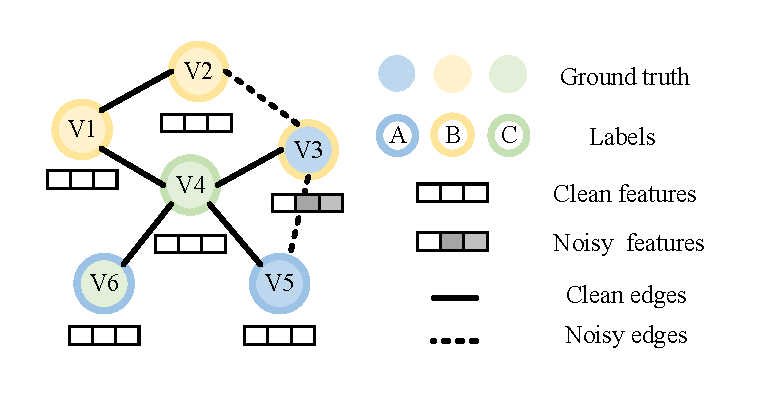
\includegraphics[width=\linewidth]{Figures/Example2.1.pdf}
      \caption{Trilateral noise}
      \Description{Node V3 introduce structural noise, feature noise, and label noise.}
      \label{fig:example}
    \end{subfigure}
    \begin{subfigure}[b]{0.17 \textwidth}
      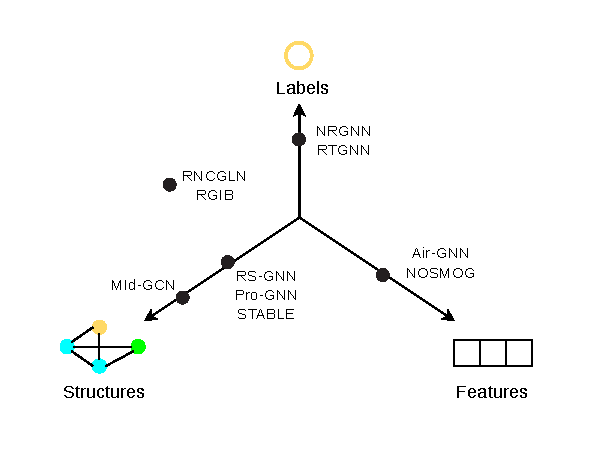
\includegraphics[width=\linewidth]{Figures/methods.pdf}
      \caption{Solution methods}
      \Description{Existing solutions on individual or corresponding noises.}
      \label{fig:methods}
    \end{subfigure}   
    \caption{Examples of trilateral noise and corresponding solution methods.}
    \Description{Figure 1. Fully described in the text.}
    \label{fig:example_and_methods}
  \end{figure}

  Existing studies typically address individual noises separately, as summarized in Figure \ref{fig:methods}. NRGNN ~\cite{dai2021nrgnn} and RTGNN ~\cite{qian2023robust} employ graph augmentation and pseudo-labeling to mitigate noisy label propagation.
  RS-GNN ~\cite{dai2022towards}, Pro-GNN ~\cite{jin2020graph} and STABLE ~\cite{li2022reliable} specifically target structural noise in graphs. Mid-GCN ~\cite{huang2023robust} designs novel convolution operations to handle  structure noise. AirGNN ~\cite{liu2021graph} and NOSMOG ~\cite{tian2022learning} purify features through graph structure. However, all these methods address a single noise type.
  In this paper, we tackle a more general and complex scenario of \textit{trilateral noise} in graph data, in which the graphs suffer from feature, structural, and label noise at the same time.

  Recent research has started to tackle the problem of robust learning in the presence of multiple types of noise. For instance,  RNCGLN ~\cite{zhu2024robust} reduces structural noise using multi-hop attention-weighted edge refinement and addresses label noise through confidence-based pseudo-labeling.  Similarly, RGIB ~\cite{zhou2023combating} handles structural and label noise using two implementations derived from the graph information bottleneck   ~\cite{wu2020graph}.  However, a common limitation among these approaches is their tendency to process different noise types through separate modules. 

  Dealing with trilateral noise (feature, structural, and label noise) presents three critical challenges:
  (1) Interconnected corruption in message passing. Feature and structural noise can introduce corrupted message passing and create error-prone dependencies between them. For instance, methods that attempt to rectify structures using features, or rectify labels using both structure and features, may generate incorrect edges or labels because the underlying information sources are themselves unreliable.
  (2) Misleading supervision and optimization. Label noise can provide misleading supervision, adversely affecting the backpropagation process. Most methods designed for correcting structural or feature noise require label supervision. When labels are incorrect, they offer flawed guidance, hindering effective optimization and leading to suboptimal graph representations. These two challenges compound each other, making learning on graphs with trilateral noise significantly more difficult.
  (3) Scalability under joint denoising. Real-world graph datasets are growing rapidly. Multi-teacher training and iterative structure-feature correction introduce extra memory overhead and computational burden. Therefore, practical robust learners are required to deliver competitive performance on large-scale graphs.


  % To address this core challenge, a feasible solution is expected to have the following properties: 
  % (1) Preventing error amplification: A significant hurdle is stopping the spread of errors.   Existing methods often attempt to correct one type of noise using information that may itself be corrupted by other noise sources, resulting in self-reinforcing error cycles.
  % (2) Designing noise-resilient correction mechanisms: It's fundamentally challenging to develop methods that can effectively correct data when trilateral noise is present, as this leaves no ``clean" source of information to reference. 

  PRINGLE ~\cite{in2024noise} attempts to address the problem of trilateral noise using a joint modeling approach. It assumes that both structural and label noise originate solely from feature noise. While this assumption simplifies the problem, it oversimplifies the complex interactions among different types of noise present in real-world settings. For example, label and structural noise may arise independently from human annotation errors and data collection faults, rather than solely from feature corruption.

  To address the above challenges, we propose \textbf{TRINA} (Trilateral noise-Robust graph learnIng for Node clAssification), a novel framework that jointly mitigates feature, structure, and label noise. To the best of our knowledge, TRINA is the first to tackle all three types of noise simultaneously without relying on oversimplified assumptions about their interactions.
  The core intuition behind TRINA is that, in a noise-free setting, node features, graph structure, and labels should exhibit mutual consistency. TRINA leverages this principle to guide both denoising and learning under noisy conditions.
  To prevent the propagation of corrupted signals during message passing, TRINA introduces a Structure-Feature Correction (SFC) module, which iteratively refines node features and graph structure based on their mutual dependencies, without assuming either modality to be clean. 
  To address misleading supervision and optimization, TRINA adopts a two-stage learning paradigm. In the first stage, multiple teacher models produce soft-label distributions and consensus pseudo-labels, reducing reliance on any single noisy signal. In the second stage, a student model is trained using these cleaner labels, enabling robust learning without noise reinforcement.
  To scale TRINA to large graphs, TRINA incorporates Metis graph partitioning~\cite{karypis1998fast} and adversarial subgraph embedding alignment~\cite{ganin2015unsupervised}, thus making it possible for each partition can be trained under limited memory while embeddings remain consistent across partitions.
  Our main contributions are as follows:
  \begin{itemize}
    \item We present the first framework to jointly address feature, structure, and label noise without relying on error-prone dependencies or strong assumptions about the noise sources.
    \item We propose a mutual structure-feature correction module that performs iterative, cross-modal denoising of graph topology and node features.
    \item We design a multi-teacher, single-student architecture that produces robust pseudo-labels and soft-label distributions, enabling reliable supervision even under heavy noise.
    \item We extend TRINA to large graphs via Metis partitioning and adversarial subgraph embedding alignment, enabling scalable training while preserving trilateral-noise robustness.
  \end{itemize}

\section{Related Work}
  \subsection{Single-source noise}
    \subsubsection{Feature noise.}
    Existing methods for correcting noisy node features typically rely on clean structural information to guide denoising. For example, NOSMOG ~\cite{tian2022learning} addresses the misalignment by complementing node content with position features to capture the graph structural information, and designs an innovative representational similarity distillation strategy. AirGNN ~\cite{liu2021graph}  designs a message passing scheme with a homophily assumption on graph
    structure data and residual connection. Besides, GTrans ~\cite{jin2022empowering} proposes a graph transformation framework that adapts and refines graph data at test time to achieve better performance. GCORNs ~\cite{abbahaddou2024bounding} uses the weight matrix to handle feature noise.
    
    \subsubsection{Structure noise.}
    Structural noise correction typically involves refining the graph topology while leveraging node features and various learning strategies. RSGNN~\cite{dai2022towards} learns to connect feature-similar nodes, and STABLE~\cite{li2022reliable} builds a denoised kNN graph. Mid-GCN~\cite{huang2023robust} filters out noise using mid-frequency components, whereas EvenNet~\cite{lei2022evennet} improves robustness through modified message passing. Other methods adjust edge reliability via weighting~\cite{jo2023robust, chen2025l2m}, edge pruning~\cite{song2023rge}, or contrastive learning~\cite{zhuang2025refine}. Recent work also explores using large language models to edit noisy graph structures~\cite{guo2024graphedit}.
    
    \subsubsection{Label Noise.}
    Label noise is typically addressed by enhancing supervision through pseudo-labeling, clean sample selection, or structural refinement. Recent methods for graph label noise include contrastive learning~\cite{li2024contrastive, lu2024noise, yuan2023learning, qian2024rlgnn}, sample scoring for clean label selection~\cite{wu2024mitigating, li2023graphcleaner, qian2023robust, dai2021nrgnn}, singular value decomposition~\cite{yuan2023alex}, and subgraph-based approaches~\cite{yin2024sport}.
    
    However, all of the above methods are designed under the assumption of single-source noise and are not directly applicable in scenarios of trilateral noise.
    
  \subsection{Multi-sources noise}
    Only a few existing methods explicitly address scenarios involving multi-source noise in graph data.  RNCGLN~\cite{zhu2024robust} targets structural and label noise by leveraging multi-hop edge information with an attention mechanism for edge reweighting, followed by pseudo-labeling to mitigate label noise. SRGNN~\cite{yuan2023self} addresses structural and label noise independently, refining graph structure through node features and using pseudo-labels for robust supervision. RGIB~\cite{zhou2023combating} tackles edge-level structural and label noise via graph augmentation and clean signal extraction, grounded in the graph information bottleneck principle. 
    However, these methods still handle each noise type separately.

    PRINGLE ~\cite{in2024noise} stands out as a unique method designed to handle trilateral noise, which encompasses corruption in node features, graph structure, and labels. It introduces a feature-driven generative noise hypothesis (FDGN), modeling both structural and label noise as originating from feature noise. This causal perspective then guides a joint denoising process. However, a notable limitation of PRINGLE is its reliance on strong assumptions that both structural and label noise originate solely from feature noise, which can restrict its applicability across diverse real-world scenarios. 

  \subsection{Large Graph Training}
    Scaling GNNs to large graphs typically relies on graph partitioning or sampling to reduce per-step memory. Metis multilevel partitioning~\cite{karypis1998fast} minimizes edge cuts under balance constraints, and Cluster-GCN~\cite{chiang2019cluster} exploits such partitions to restrict neighborhood aggregation within dense clusters. Complementary to partitioning, adversarial learning with a gradient reversal layer~\cite{ganin2015unsupervised} is widely used to align feature distributions across domains. Nevertheless, existing scalable training pipelines rarely address feature, structure, and label noise jointly. TRINA couples trilateral-noise robust learning with Metis partitioning and adversarial subgraph alignment to remain effective at large scale.

\section{Problem Definition}
  \begin{definition}[Graph]
    A graph $\mathcal{G}$ is defined as a tuple $\langle\mathcal{V}, \mathcal{E}, \mathcal{X}\rangle$, where $\mathcal{V} = \{v_{1}, \dots, v_{N}\}$ is the set of nodes, $\mathcal{E} \subseteq \mathcal{V} \times \mathcal{V}$ is the set of edges, and $\mathcal{X} \in \mathbb{R}^{N \times F}$ represents the node feature matrix, with $F$ being the number of features. Each node $v_i$ is associated with a feature vector $\mathcal{X}_{i} \in \mathbb{R}^{F}$ and a one-hot encoded label $y_i \in \{0,1\}^{C}$, where $C$ is the number of classes. The observed graph structure is represented by an adjacency matrix $\mathbf{A} \in \mathbb{R}^{N \times N}$, where $\mathbf{A}_{ij} = 1$ if there exists an edge between $v_i$ and $v_j$, and $\mathbf{A}_{ij} = 0$ otherwise.
  \end{definition}

  \begin{definition}[Trilateral Noise Graph]
    A trilateral noise graph is one that is simultaneously corrupted by noise in its labels, structure, features:
    (1) Label Noise: The provided labels $\mathcal{Y}$ for $\mathcal{V}_{L}$ are corrupted versions of the true labels.
    (2) Structure Noise: The observed adjacency matrix $\mathcal{A}$ deviates from the true graph structure.
    (3) Feature Noise: The observed node features $\mathcal{X}$ are noisy variants of the true features.
  \end{definition}

  \begin{definition}[Node Classification]
    Given a graph $\mathcal{G} = \langle\mathcal{V}, \mathcal{E},$ $ \mathcal{X}\rangle$, the node set is divided into a labeled subset $\mathcal{V}_{L}$ and an unlabeled subset $\mathcal{V}_{U} = \mathcal{V} \setminus \mathcal{V}_{L}$. The objective is to train a model using the labeled nodes in $\mathcal{V}_{L}$, in order to accurately predict the true labels of nodes in $\mathcal{V}_{U}$.
  \end{definition}

  Our objective is to solve the node classification problem in a trilateral noise graph:

\begin{figure*}
  \centering
  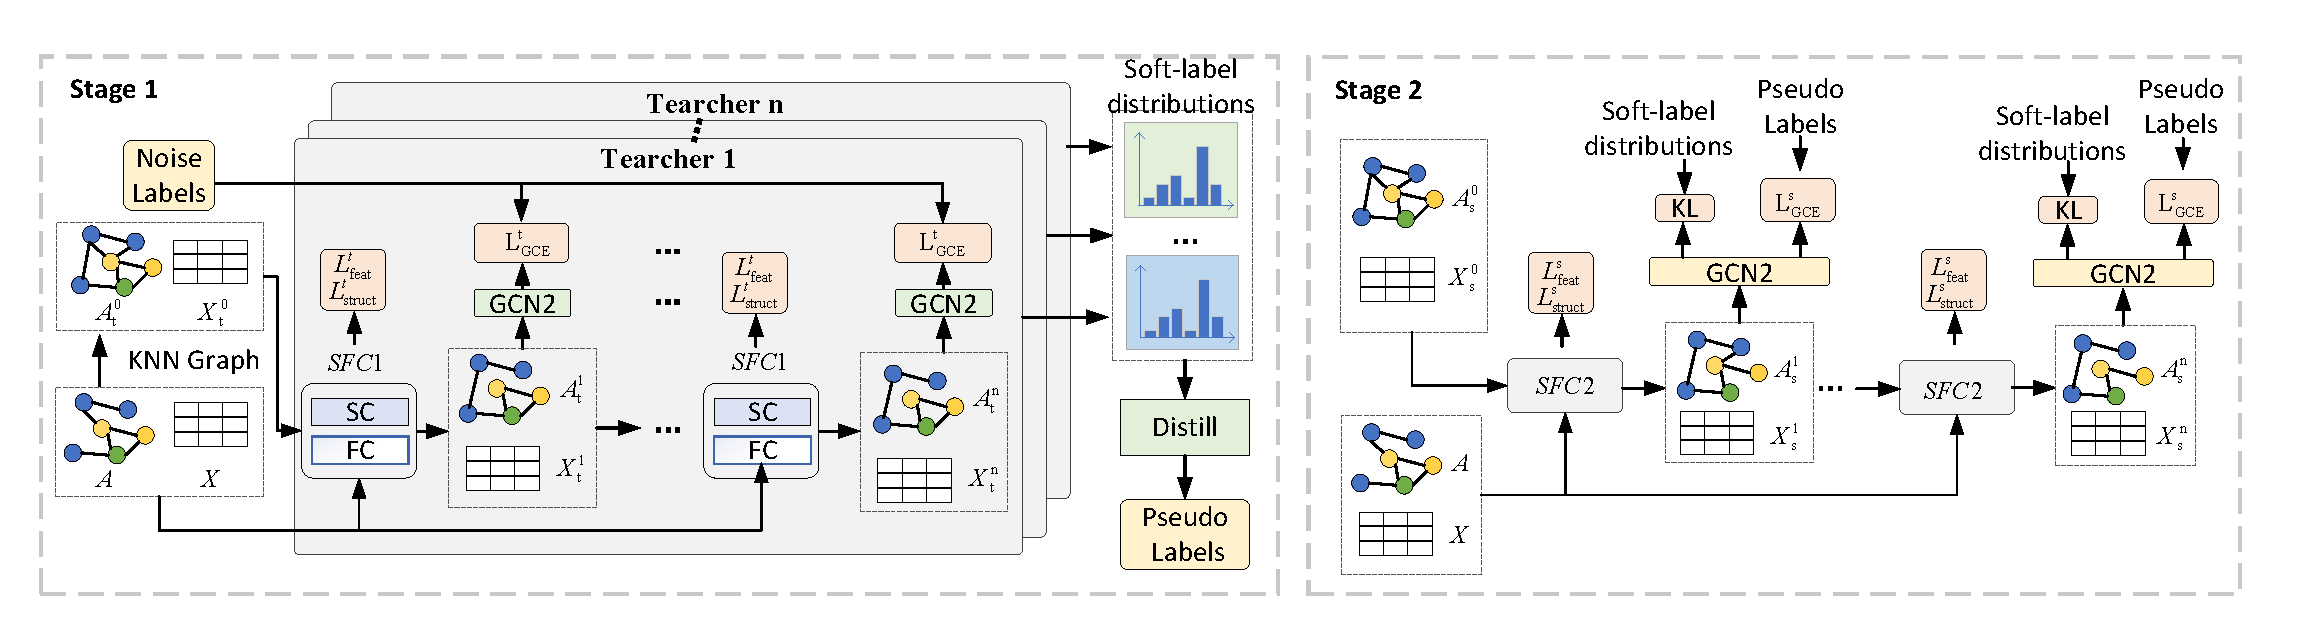
\includegraphics[width=\linewidth]{Figures/framework.pdf}
  \caption{The two-stage architecture: 
  (1) Stage 1 trains teacher models; 
  (2) Stage 2 trains student model for final classification.}
  \Description{Figure 2. Fully described in the text.}
  \label{fig:overall_architecture}
\end{figure*}

\section{Methodology}
  \subsection{Framework Overview}
    % In practice, it is very likely that features, structure, and labels are mutually consistent in the absence of noise. 
    % \st{To address this issue, we propose a multi-stage purification framework that iteratively refines each noisy component by leveraging the mutual dependencies among them.}
    % To address the core challenges of error amplification and intertwined noise, we propose a two-stage framework designed to decouple the complex learning process. The fundamental idea is to separate the task of generating a reliable supervisory signal from the final classification task. 
    As mentioned in the introduction, addressing noise in features, graph structure, and labels presents two primary challenges: interconnected corruption and misleading supervision.
    We address corruption in both features and graph structure using the Structure-Feature Correction (SFC) module, which iteratively refines them by modeling their mutual dependencies. In each training epoch, the SFC module corrects the graph structure and features by referencing both the original and the previous epoch's graph. This prevents the model from straying too far from the initial data while still progressively cleaning the graph. Consequently, each epoch yields a cleaner, more reliable graph representation.
    Building on SFC, we propose a teacher-student architecture trained in two stages to address the misleading supervision issue. The first stage leverages an ensemble of teacher models to distill robust, consensus-based pseudo-labels, effectively filtering the initial label noise. In the second stage, a student model learns from this purified supervisory label. 
    The design is motivated by the observation that, in clean settings, features, structure, and labels tend to be mutually consistent. By encouraging this consistency during training, TRINA progressively aligns the learning process toward a noise-free solution.
    The overall architecture is illustrated in Figure~\ref{fig:overall_architecture}.
    On medium-sized graphs we train TRINA over the full graph; on large graphs we enable the Metis partitioning and adversarial alignment extension.

    In the following subsection, we first present the structure of Structure-Feature Correction module, which aims to address the noises in structure and feature. Then, we introduce the Teacher-Student architecture, aiming to address the noises in the label. Finally, we describe how TRINA scales to large graphs.

  \subsection{Structure-Feature Correction (SFC) Module}\label{sec:sfc}
    The Structure and Feature Correction (SFC) module serves as a fundamental building block for denoising both graph structure and node features. It consists of two parallel submodules: the Structural Cleaning (SC) submodule and the Feature Cleaning (FC) submodule, which are responsible for refining the adjacency matrix and denoising the node features, respectively.

    In both the teacher and student models, the SFC module takes four inputs: the original adjacency matrix and node feature matrix, along with a purified adjacency matrix and purified node feature matrix from the previous training epoch. Based on these inputs, the SFC module produces updated (i.e., more purified) versions of the adjacency matrix and node features, which are then used in the subsequent epoch to progressively enhance the graph structure and node features. For the first training epoch, since no purified information from a previous epoch is available, we initialize the purified adjacency matrix using a K-Nearest Neighbor (KNN) graph constructed from the original node features, and set the purified feature matrix to be identical to the original feature matrix. We next elaborate on the SC submodule and FC submudule in details.

    \subsubsection{Structural Cleaning (SC)}
      The Structural Cleaning (SC) submodule progressively refines a graph's structure throughout the training process. 
      It addresses potential inaccuracies in the initial K-Nearest Neighbors (KNN) graph, which is constructed from noisy feature data. To correct this, SC iteratively improves the graph by using progressively cleaner node representations to identify and remove erroneous connections. To prevent going too far and removing correct edges, we've designed a structure loss. Simultaneously, a noise-robust loss offers flexible supervision, preventing the SC submodule's structural refinements from deviating excessively from the available label information.
      
      Specifically, at each epoch $i$, SC takes three inputs: the original adjacency matrix $\mathbf{A}_o$, node features matrix from the previous epoch  $\mathbf{X}_t^{i-1}$ and adjacency matrix from the previous epoch  $\mathbf{A}_t^{i-1}$.

      First, the original adjacency matrix $\mathbf{A}_o$ and the updated node features from the previous epoch $\mathbf{X}_t^{i-1}$ are fed into a GCN to compute node representations:
      \begin{equation}
        \label{eq:rep}
        \mathbf{H} = \text{GCN1}(\mathbf{A}_o, \mathbf{X}_t^{i-1}).
      \end{equation}

      Next, to adaptively fuse the initial and previous adjacency matrices and prevent the graph deviating excessively from its original topology, a learnable binary mask $\mathbf{W_1} \in \{0,1\}^{n \times n}$ is introduced:
      \begin{equation}
        \mathbf{A}_{\text{fused}} = \mathbf{W_1} \odot \mathbf{1}_{\mathbf{A}_t^{0}\neq 0}  + (\mathbf{1} - \mathbf{W_1}) \odot \mathbf{1}_{\mathbf{A}_t^{i-1}},
      \end{equation}
      where $\odot$ denotes element-wise multiplication, $\mathbf{1}$ is an all-ones matrix, and $\mathbf{1}_{A\neq 0}$ returns 1 if the condition is non-zero  and 0 otherwise. 
      For each candidate edge $(v_i,v_j)$ in $\mathbf{A}_{\text{fused}}$ (i.e., $\mathbf{A}_{\text{fused}}[i][j] \neq 0$), an edge confidence score is calculated using node embeddings:
      \begin{equation}
        p_{j,k} = \sigma(sim (\mathbf{H}[j], \mathbf{H}[k])),
      \end{equation}
      where $\text{sim}(\cdot,\cdot)$ denotes cosine similarity and $\sigma$ is the ReLU activation function.

      The refined adjacency matrix $\mathbf{A}_t^{i}$ is then constructed by retaining only those edges whose confidence score exceeds a predefined threshold $\tau$:
      \begin{equation}
        \label{eq:Ati}
        \mathbf{A}_t^{i}[j][k] =
        \begin{cases}
          p_{j,k} & \text{if } \mathbf{A}_{\text{fused}}[j][k] \neq 0 \text{ and } p_{j,k} > \tau, \\
          0 & \text{otherwise}.
        \end{cases}
      \end{equation}

      The resulting structure $\mathbf{A}_t^{i}$  serves as the input adjacency matrix for the subsequent epoch  $i+1$.

      To ensure that the model retains essential connectivity patterns while filtering out noisy or irrelevant connections, we introduce a structure reconstruction loss:
      \begin{equation}
        \begin{aligned}
          \mathcal{L}^t_{\text{struct}}
          &= \frac{N}{|\mathcal{E}^+| + |\mathcal{E}^-|}
          \Biggl[
            \sum_{(v_j,v_k) \in \mathcal{E}^+}
            \bigl( p_{j,k}^{\text{reg}} - 1 \bigr)^2 \\
          &\qquad
            + \sum_{(v_j,v_k) \in \mathcal{E}^-}
            \bigl( p_{j,k} - 0 \bigr)^2
          \Biggr],
        \end{aligned}
      \end{equation}
      where $N$ is the number of nodes, and $\mathcal{E}^+$ and $\mathcal{E}^-$  represent the sets of positive (existing) and randomly sampled negative (non-existing) edges, respectively.
      The regularized prediction $p_{jk}^{\text{reg}}$ is computed as:
      \begin{equation}
        p_{j,k}^{\text{reg}} = \theta \cdot \text{sim}(\mathcal{X}[j], \mathcal{X}[k]) + (1 - \theta) \cdot p_{j,k},
      \end{equation}
      where $p_{j,k}^{\text{reg}}$  is a weighted average of the original predicted probability and the cosine similarity of the nodes' original features,  $\text{sim}(\mathcal{X}[j], \mathcal{X}[k])$. The hyperparameter  $\theta \in [0,1]$
      controls the balance between these two components.
      This regularization is applied to positive edges to reinforce their validity using feature similarity, thereby mitigating the impact of noisy connections that might exist in the ground-truth graph. For negative edges, we directly use 
      $p_{j,k}$ since they are randomly sampled and assumed to be false. 

    \subsubsection{Feature Cleaning.}
      The Feature Cleaning (FC) submodule aims to iteratively suppress feature noise during training. Because the initial input features may be corrupted, FC reconstructs each node’s representation using its neighborhood information to identify and correct noisy features. At each epoch, nodes whose features significantly deviate from their reconstructed counterparts,  are considered noisy and corrected accordingly.  The underlying intuition is that normal nodes are usually similar to their neighbors, while noisy nodes tend to deviate from this local consistency.
      To prevent excessive modification of the features, a penalized feature reconstruction error loss is introduced to limit the degree of change. Additionally, a noise robust loss provides adaptive supervision.

      At each epoch $i$, the module takes three inputs: the features from the previous epoch $\mathbf{X}_t^{i-1}$, the original input adjacency matrix $\mathbf{A}_o$ the original input features $\mathbf{X}_o$.
      To balance the preservation of raw input information and the refinement from previous epochs, the module first fuses $\mathbf{X}_t^{i-1}$ and $\mathbf{X}_o$ using an adaptive interpolation strategy.  Specifically, a learnable weight matrix $\mathbf{W_2} \in [0,1]^{n \times d}$ is used to control the contribution of each feature dimension:
      \begin{equation}
        \mathbf{X}_{\text{fused}} = \mathbf{W_2} \odot \mathbf{X}_t^{i-1} + (\mathbf{1} - \mathbf{W_2}) \odot \mathbf{X}_o,
      \end{equation}
      where $\odot$ denotes the Hadamard product and $\mathbf{1}$ represents an all-ones matrix.
      The fused features $\mathbf{X}_{\text{fused}}$ are then passed into GraphMAE~\cite{hou2022graphmae}, a graph masked autoencoder that leverages the original adjacency matrix $\mathbf{A}_o$ to perform structure-aware reconstruction.
      \begin{equation}
        \mathbf{X}'_{\text{fused}} = \text{GraphMAE}(\mathbf{A}_o, \mathbf{X}_{\text{fused}}).
      \end{equation}
      To prevent trivial identity mapping and encourage meaningful learning, GraphMAE randomly selects a subset of nodes $\tilde{\mathcal{V}} \subset \mathcal{V}$ and replaces their features with a learnable mask token $x_{[M]} \in \mathbb{R}^F$:
      \begin{equation}
        \tilde{\mathbf{X}}_{\text{fused}}[i] =
        \begin{cases}
          x_{[M]}&v_i \in \tilde{V},\\
          \mathbf{X}_{\text{fused}}[i]& v_i \notin \tilde{V}.
        \end{cases}
      \end{equation}
      
      The masked feature matrix $\tilde{\mathbf{X}}_{\text{fused}}$ is then input to the graph autoencoder, producing reconstructed features $\mathbf{X}'_{\text{fused}}$. Although this masking strategy promotes robust feature learning, it can create a mismatch between training and inference since masked tokens do not appear during deployment.
      
      The FC module adopts the Scaled Cosine Error (SCE) loss~\cite{hou2022graphmae}, which penalizes reconstruction errors with an exponential scaling factor $\gamma > 1$:
      \begin{equation}
        \mathcal{L}^t_{\text{feat}} = \frac{1}{|\tilde{\mathcal{V}}|} \sum_{v_i \in \tilde{\mathcal{V}}} \left(1 - \frac{\mathbf{X}'_{\text{fused}}[i] \cdot \mathbf{X}_o[i]}{|\mathbf{X}'_{\text{fused}}[i]| \cdot |\mathbf{X}_o[i]|} \right)^\gamma.
      \end{equation}

      This loss accentuates difficult reconstruction cases and helps the model focus on noisy or corrupted features for subsequent correction.

      To identify noisy nodes, the module calculates the element-wise reconstruction error using the L1 norm:
      \begin{equation}
        \Delta = |\mathbf{X}' - \mathbf{X}_{o}|.
      \end{equation}

      The top-$k$ nodes with the highest error scores in $\Delta$ are selected as the noisy set, $\mathcal{V}_{\text{noisy}}$.
      The assumption is that nodes with a large difference between their original and reconstructed features are likely to be corrupted or uninformative.

      For each node $v_k \in \mathcal{V}_{\text{noisy}}$, its feature vector is corrected by replacing it with the average of its neighbors' feature vectors from the previous epoch. This can be expressed as:
      \begin{equation}
        \mathbf{X}^i_t[k] = \frac{1}{|\mathcal{N}(v_k)|} \sum_{v_j \in \mathcal{N}(v_k)} \mathbf{X}^{i-1}_t[j],
      \end{equation}
      where $\mathcal{N}(v)$ denotes the set of neighbors of node $v$ in $\mathbf{A}_o$.
      This updated feature matrix is then used as input for the next epoch, allowing the model to progressively denoise features over time.

  \subsection{Training the Teacher-Student Architecture}\label{sec:teacher_student}
    To address the label noise, we employs a multi-teacher single-student architecture ~\cite{huang2021multi}, drawing inspiration from effective knowledge distillation techniques ~\cite{li2022learning}. 
    \subsubsection{Training of teacher models.}
      The teacher models are trained independently with different initializations to encourage diversity. Specifically, in a teacher model, the purified node features $\mathbf{X}_{t}^{i}$ and adjacency matrix $\mathbf{A}_{t}^{i}$ at epoch $i$ are fed into a GNN-based predictor to generate label predictions $\hat{\mathbf{Y}}$. This predictor, an implementation of a weighted Graph Convolutional Network (GCN) ~\cite{kipf2016semi}, employs layer-wise propagation:
      \begin{equation}
        \mathbf{H}^{(i)} = \text{GCN2}(\mathbf{A}_{t}^{i}, \mathbf{X}_{t}^{i}).
      \end{equation}

      Subsequently, a softmax output layer converts these representations into class probability distributions:
      \begin{equation}
        \hat{\mathbf{Y}} = \text{softmax}(\mathbf{H}^{(i)}),
      \end{equation}
      where $\hat{\mathbf{Y}} \in \mathbb{R}^{|\mathcal{V}|\times C}$, where $C$ is the number of classes, and  each entry $\hat{y}_{v,c}$ denotes the predicted probability of node $v$ belonging to class $c$.

      To enhance robustness against label noise, we adopt the Generalized Cross Entropy (GCE) loss ~\cite{zhang2018generalized}, which bridges the noise tolerance of mean absolute error and the optimization efficiency of standard cross entropy.
      For multi-class classification with a one-hot ground-truth vector 
      $y_v=\{y_{v,1},\dots, y_{v, C}\}$,   the GCE loss is defined as:
      \begin{equation}
        \mathcal{L}^t_{\text{GCE}} = \frac{1}{q} \sum_{v \in \mathcal{V}} \sum_{c=1}^C y_{v,c} \left(1 - \hat{y}_{v,c}^q\right),
      \end{equation}
      where $q \in (0,1]$ controls the trade-off between robustness and sensitivity, $y_c$  indicates whether class  $c$ is the true label of node 
      $v$. 

      The overall training loss for a teacher model at each epoch is a composite of three terms: structure, features, and label supervision:
      \begin{equation}
        \mathcal{L}_{total}^{t} = \lambda_1\mathcal{L}^t_{\text{GCE}}+\lambda_2\mathcal{L}^t_{\text{struct}} + \lambda_3\mathcal{L}^t_{\text{feat}}.
      \end{equation}

    \subsubsection{Training of student model.}
      Once all teacher models have been trained, they potentially specialize in different aspects of noise patterns. We next train the student model to synthesize more comprehensive knowledge by learning from multiple teachers. This ultimately leads to better generalization than any single teacher could achieve alone.

      Let $\hat{\mathbf{Y}}_k$ denote the predicted probability distributions from the $k$-th teacher. To transfer soft knowledge, the student minimizes the KL divergence between its predictions and those from each teacher:
      \begin{equation}
        \mathcal{L}^s_{\text{KLD}} = \sum_{k=1}^K  \sum_{v\in \mathcal{V}}\text{KL}\left(\hat{Y}_k^{v} \parallel \hat{Y}_{\text{student}}^{v}\right),
      \end{equation}
      where $\hat{Y}_k^{v}$ and $\hat{Y}_{\text{student}}^{v}$ denote the predicted class probability distributions for node $v$ from the $k$-th teacher and the student model, respectively.

      Beyond soft label alignment, we further purify supervision by extracting high-confidence samples. A node $v$ is deemed clean by the $k$-th teacher if the highest predicted probability exceeds a confidence threshold $\tau$:
      \begin{equation}
        \mathcal{C}_k = \left\{ v \in \mathcal{V} \mid \max(\hat{Y}_k^{v}) > \tau \right\}.
      \end{equation}

      Here, $\hat{Y}_k^{v}$ represents the predicted probability distribution of node  $v$ by the $k$-th teacher. Then, the set of high-confidence samples from all teachers is:
      %Nodes in $\mathcal{C}$ are treated as high-confidence supervision anchors. The student is supervised on these nodes via GCE loss:
      \begin{equation}
        \mathcal{C} = \bigcap_{k=1}^n \mathcal{C}_k.
      \end{equation}

      Nodes in the set $\mathcal{C}$ serve as high-quality supervision sources, guiding the student model to jointly mitigate both structural and feature-level noise. The hard label loss is shown as:
      \begin{equation}
        \mathcal{L}^s_{\text{GCE}} = \frac{1}{q} \sum_{v \in \mathcal{C}} \sum_{c=1}^C y_{v,c} \left(1 - \hat{y}_{v,c}^q\right).
      \end{equation}

      By integrating soft label distillation and hard label correction, the student model benefits from both generalized knowledge transfer and noise-resistant supervision. The total training objective is formulated as a weighted combination of four loss components:
      \begin{equation}
        \mathcal{L}^s_{\text{total}} = \lambda_1 \mathcal{L}^s_{\text{GCE}} + \lambda_2 \mathcal{L}^s_{\text{struct}} + \lambda_3 \mathcal{L}^s_{\text{feat}} + \lambda_4 \mathcal{L}^s_{\text{KLD}},
      \label{eq:loss}
      \end{equation}
      where $\mathcal{L}^s_{\text{struct}}$ and $\mathcal{L}^s_{\text{feat}}$ are computed in the same way as their teacher counterparts, i.e., $\mathcal{L}^t_{\text{struct}}$ and $\mathcal{L}^t_{\text{feat}}$. Note that the KLD term is omitted during teacher training (i.e., $\lambda_4 = 0$), while the student model optimizes all four terms. This multi-objective learning strategy preserves graph structure, suppresses feature and label noise, and effectively distills complementary knowledge from the teacher ensemble for enhanced robustness.

  \subsection{Scaling to Large Graphs}\label{sec:large}
    Applying TRINA directly to large graphs will face multiple realistic constraints: adjacency matrix surge with the number of nodes, SFC iterative denoising and multi-teacher integration bring high computational overhead. Ordinary subgraph sampling will lose neighborhood information and destroy the edge confidence estimation of the SC module. 
    Thus, we extend the model based on Metis~\cite{karypis1998fast} graph partitioning combined with adversarial subgraph embedding alignment~\cite{ganin2015unsupervised}. 
    Metis partition can balance the size of subgraphs, reducing edge loss across partitions, and is suitable for splitting the original graph. 
    Adversarial alignment specifically alleviates the distribution shift of subgraph representation caused by partitioning, ensuring the consistency of embedding space after splitting training, and completely retains all three-party noise denoising capabilities of TRINA.
    Details are illustrated in Figure~\ref{fig:large_scale}.
    
    \begin{figure}[t]
      \centering
      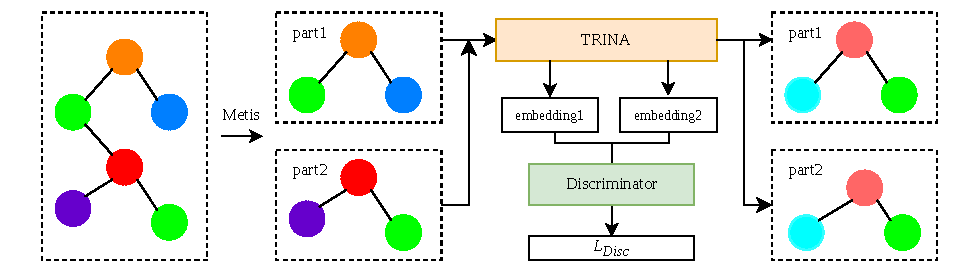
\includegraphics[width=1.0\linewidth]{Figures/large_scale_graph_extention.pdf}
      \caption{Large-scale extension of TRINA: Metis partitions the graph and adversarial discriminator aligns embeddings.}
      \Description{Figure 3. Fully described in the text.}
      \label{fig:large_scale}
    \end{figure}

    \subsubsection{Metis Graph Partitioning.}
      We partition the original graph $\mathcal{G}=(\mathcal{V},\mathcal{E},\mathcal{X})$ into $P$ subgraphs $\{G_k=(A_k,X_k)\}_{k=1}^{P}$ using Metis multilevel partitioning~\cite{karypis1998fast}. Let $\Pi=\{\mathcal{V}_1,\ldots,\mathcal{V}_P\}$ denote a partition of the node set. Metis approximately minimizes the cross-partition edge cut subject to a load-balance constraint that keeps partition sizes comparable:
      \begin{equation}
        \mathrm{cut}(\Pi) = \sum_{1 \le a < b \le P}
        \sum_{u \in \mathcal{V}_a,\, v \in \mathcal{V}_b} \mathbf{A}_{uv},
        \quad |\mathcal{V}_k| \approx \frac{|\mathcal{V}|}{P}.
      \end{equation}
      Compared with random cuts, Metis better preserves local community structure that message passing relies on. Each subgraph then runs the same SFC module and teacher--student training as in the full-graph setting.

    \subsubsection{Adversarial Subgraph Embedding Alignment.}
      Different partitions may exhibit distinct topology densities and community statistics, inducing subgraph-specific embedding shifts that hurt cross-partition generalization. Viewing each partition as a domain, we introduce a multilayer perceptron (MLP) discriminator $D_{\phi}$ and train the GNN encoder $f_{\theta}$ adversarially so that embeddings become partition-invariant~\cite{ganin2015unsupervised}.

      Let $H_k=f_{\theta}(A_k,X_k)$ denote the embeddings on partition $k$, and let $h_i$ be the embedding of node $v_i$. The discriminator outputs a categorical distribution over the $P$ partitions,
      \begin{equation}
        p_i = D_{\phi}(h_i) = \mathrm{softmax}\bigl(\mathrm{MLP}(h_i)\bigr) \in \mathbb{R}^{P},
      \end{equation}
      where the $m$-th entry $p_i^{(m)}$ is the predicted probability that $v_i$ belongs to partition $m$. Given the true partition label $y_i\in\{0,1\}^{P}$, the discriminator is trained by minimizing the multi-class cross-entropy:
      \begin{equation}
        \mathcal{L}_{\text{disc}} = - \sum_{v_i \in \mathcal{V}} \sum_{m=1}^{P} y_i^{(m)} \log p_i^{(m)}.
      \end{equation}
      A stronger discriminator indicates that embeddings still carry partition-specific bias. Conversely, if $f_{\theta}$ succeeds in aligning distributions across partitions, $D_{\phi}$ becomes harder to train.

      Let $\mathcal{L}_{\text{task}}$ denote the original TRINA training loss on each subgraph. We couple the task objective with adversarial alignment and optimize the two networks alternately:
      \begin{equation}
        \min_{\phi}\; \mathcal{L}_{\text{disc}},
        \qquad
        \min_{\theta}\; \mathcal{L}_{\text{task}} - \lambda_a \mathcal{L}_{\text{disc}},
      \end{equation}
      where $\lambda_a$ balances task learning and partition invariance. In each training round, we first fix the encoder parameters $\theta$ and update only the discriminator parameters $\phi$ to better identify partition origins; we then fix $\phi$ and update $\theta$ through a gradient reversal layer (GRL), which flips the sign of $\partial \mathcal{L}_{\text{disc}}/\partial \theta$ so that the encoder confuses $D_{\phi}$.

  \subsection{Time Complexity.}
    The total training complexity of the teacher model and the student model per epoch is the sum of the computational costs of SFC and the subsequent GCN classifier. SFC involves two parallel submodules SC and FC. The complexity of SC is $O(|V|\cdot d^2 + (|E| + |E_{\text{fused}}|)\cdot d)$, where $|V|$ is the number of nodes, $|E|$ is the number of edges in the original graph, $|E_{\text{fused}}|$ is the number of edges in the fused graph, and $d$ is the feature dimension. FC's complexity is determined by the GraphMAE component, leading to a cost of $O(|V|\cdot d^2 + |E|\cdot d)$. The GCN classifier's complexity is $O(|V|\cdot d^2 + |E_{\text{purified}}|\cdot d)$, where $|E_{\text{purified}}|$ is the number of edges in the purified graph for the current epoch. By assuming $|E|$, $|E_{\text{fused}}|$ and $|E_{\text{purified}}|$ are on the same order of magnitude, the complexity for training a teacher/student model per epoch on a full graph is $O(|V|\cdot d^2 + |E|\cdot d)$.

    For large graphs with $P$ Metis partitions (e.g., $P{=}4$ on ogbn-arxiv), each partition contains roughly $|V|/P$ nodes and $|E|/P$ edges. Training on a single partition therefore costs about $O((|V|/P)\cdot d^2 + (|E|/P)\cdot d)$ per epoch, reducing peak memory and per-step computation by a factor of approximately $P$. The adversarial discriminator adds only a lightweight MLP classification cost that is dominated by message passing. The overall training cost is the sum of teacher/student costs over the $P$ partitions. During inference, the iterative SFC module is bypassed. The process consists of a single forward pass through the trained student GCN, with time complexity $O(|V|\cdot d^2 + |E_{\text{final}}|\cdot d)$, where $|E_{\text{final}}|$ is the number of edges in the final purified graph structure.

\section{Experiments}
  In this section, we present experimental results on real-world datasets to demonstrate the effectiveness of our proposed framework. Specifically, we investigate the following research questions:
  \begin{itemize}
    \item \textbf{RQ1} How robust is the proposed TRINA framework to trilateral noise and varying noise levels?
    \item \textbf{RQ2} Is the proposed framework robust to different noise types?
    \item \textbf{RQ3} Does each individual module of the model contribute to improved prediction accuracy?
    \item \textbf{RQ4} Does the model exhibit satisfactory computational efficiency?
  \end{itemize}
  \subsection{Experimental Settings}
    \subsubsection{Datasets.}
      \begin{table}
        \centering
        \caption{Statistics of datasets.}
        {\small
        \begin{tabular}{ccccc}
          \toprule
          Dataset & \# nodes & \# edges & \# features & \# classes \\
          \midrule
          Cora & 2708 & 5429 & 1433 & 7 \\
          Citeseer & 3312 & 4723 & 3703 & 6 \\
          Photo & 7650 & 119{,}081 & 745 & 8 \\
          Pubmed & 19{,}717 & 44{,}338 & 500 & 3 \\
          ogbn-arxiv & 169{,}343 & 1{,}166{,}243 & 128 & 40 \\
          \bottomrule
        \end{tabular}}
        \label{tab:dataset}
      \end{table}
      We evaluate the robustness of our proposed method on five datasets: three citation networks (Cora, Citeseer, and Pubmed)~\cite{sen2008collective}, one Amazon co-purchase network (Photo)~\cite{shchur2018pitfalls}, and one large-scale benchmark (ogbn-arxiv) ~\cite{hu2021ogb}. Table~\ref{tab:dataset} summarizes dataset statistics.

      Following prior work ~\cite{zhu2024robust, in2024noise, qian2023robust}, we assessed model robustness by injecting two common types of noise: uniform and pair noise. In addition, we introduced two novel noise types.
      (1) Feature-based noise: Injects noise into the k edges furthest from a node's feature representation.
      (2)  Class confusion noise: Replaces a targeted node's features with those from samples of other categories. 
      % Details are provided in the Appendix.

      We consider three distinct trilateral noise settings by varying the ratios of structure noise ($\text{gr}$), label noise ($\text{lr}$), and feature noise ($\text{fr}$). Specifically, we evaluate the model under ${\text{gr}, \text{lr}, \text{fr}} = {0, 0, 0}$ (noise-free), ${0.1, 0.1, 0.1}$ (mild noise), and ${0.3, 0.3, 0.3}$ (severe noise). This design allows for an intuitive comparison across increasing levels of corruption.

    \subsubsection{Evaluation metrics.}
      Our experiment employs two complementary metrics to assess model performance under noise:  Accuracy and F1-Macro.
      % Accuracy measures the \textit{overall classification correctness} by calculating the ratio of correctly predicted nodes to total nodes.F1-macro computes the \textit{unweighted mean} of per-class F1-scores, where each class contributes equally regardless of sample size.

    \subsubsection{Baselines.}
      The comparison methods include GCN ~\cite{kipf2016semi}, which does not address either graph noise or label noise; two multi-noise robust methods, RNCGLN ~\cite{zhu2024robust} and PRINGLE ~\cite{in2024noise}; one label-noise robust method, RTGNN ~\cite{qian2023robust}; and one graph-noise robust method, Mid-GCN ~\cite{huang2023robust}.  Details are provided in the Appendix.

    \subsubsection{Implementation Details.}
      Both the teacher and student SC modules adopt a single-layer GCN with 128 hidden units (denoted as GCN1) as the encoder. Their prediction models are implemented as two-layer GCNs with 128 hidden units (denoted as GCN2). The hyperparameter   \(\tau\) in Eq.~\ref{eq:Ati} is set to $0.05$ across all datasets. We fix the loss weights as \(\lambda_1 = 1\), \(\lambda_2 = 0.03\), \(\lambda_3 = 1\), \(\lambda_4 = 300\); for teacher models, the KLD term is disabled by setting 
      \(\lambda_4 = 0\).
      We perform hyperparameter search for the number of nearest neighbors \(K\) in $k$-nearest neighbor (KNN) graph from the set 
      \(\{50, 100, 200, 400, 600, 800\}\) based on the validation performance. The number of teacher models is fixed at $4$.
      The model is trained for 2000 epochs using the Adam optimizer with a learning rate of \(5 \times 10^{-4}\) and a weight decay of \(5 \times 10^{-4}\). To prevent overfitting, we apply dropout with a rate of  \(0.5\), and adopt early stopping. All reported results are averaged over $4$ independent runs.
      On medium-sized datasets we train TRINA on the full graph without partitioning or adversarial alignment. On ogbn-arxiv, we enable the large-graph extension: Metis partitions the graph into $4$ subgraphs, the KNN neighborhood size is set to $K{=}200$, and the adversarial alignment weight is $\lambda_a{=}0.1$. KNN graph construction is accelerated by FAISS~\cite{johnson2019billion}.

  \subsection{Performance Comparison (RQ1 and RQ2)}
    This section compares the performance of all methods across different levels and types of noise.
    \subsubsection{Performance on Different Levels of Trilateral Noise.} 
      Table \ref{tab:performence_uniform} presents node classification results under uniform trilateral noise, demonstrating TRINA’s state-of-the-art performance. GCN shows significant performance degradation as noise increases, while methods designed for single noise types such as RT-GNN and Mid-GCN exhibit some robustness but remain less effective than multi-noise approaches. Multi-noise methods like RNCGLN and PRINGLE generally perform well but occasionally underperform. For example, RNCGLN scored lower than GCN on CiteSeer and Photo at noise level ${0.3,0.3,0.3}$, and PRINGLE performed worse than Mid-GCN on Pubmed under the same noise conditions. In contrast, TRINA consistently achieves the highest or near highest accuracy and F1 macro scores. Notably, at noise level ${0.3,0.3,0.3}$, TRINA outperforms the second best method by $7.85$ percent on Cora and by $8.6$ percent on Pubmed.
      On the large-scale ogbn-arxiv benchmark, TRINA remains the strongest method across all noise levels. At noise level ${0.3,0.3,0.3}$, TRINA improves accuracy by $5.04$ percentage points over the second-best baseline PRINGLE, indicating that Metis partitioning with adversarial alignment preserves TRINA's robustness at scale.
      \begin{table*}
        \centering
        \caption{Performance Comparison w.r.t uniform noise (Accuracy(\%)±Std \& F1 Macro Score)}        
        {\small
        \begin{tabular}{ccccccccc}
          \toprule
          Dataset&Metrics&\{gr,lr,fr\} & GCN & Mid-GCN & RT-GNN & PRINGLE & RNCGLN & TRINA\\
          \midrule
          \multirow{6}{*}{Cora}& \multirow{3}{*}{Accuracy}&\{0,0,0\}&84.26±0.52&\underline{84.50±0.70}&78.02±0.31&83.13±0.09&83.11±0.70&\textbf{85.19±0.86} \\
            &&\{.1,.1,.1\}&73.53±0.13&73.82±0.29&71.57±0.37&\underline{77.95±0.23}&75.59±1.59&\textbf{81.33±0.32}  \\
            &&\{.3,.3,.3\}&54.02±0.45&57.70±0.42&58.81±0.98&61.60±0.58&\underline{65.33±0.62}&\textbf{73.18±1.00 }\\
            
              & \multirow{3}{*}{F1 Score}&\{0,0,0\}&\underline{0.83±0.00}&\underline{0.83±0.00}&0.69±0.00&0.82±0.00&0.81±0.01&\textbf{0.84±0.00} \\
            &&\{.1,.1,.1\}&0.72±0.00&0.72±0.00&0.64±0.01&\underline{0.77±0.00}&0.73±0.02&\textbf{0.81±0.00} \\
            &&\{.3,.3,.3\}&0.50±0.01&0.53±0.02&0.29±0.22&0.60±0.01&\underline{0.63±0.00}&\textbf{0.73±0.01}\\
          
          \midrule
          \multirow{6}{*}{CiteSeer}& \multirow{3}{*}{Accuracy} &\{0,0,0\}&67.98±0.62&70.55±0.45&67.58±1.54&\underline{71.40±1.63}&70.63±1.11&\textbf{72.38±0.89} \\
            &&\{.1,.1,.1\}&68.23±1.22&61.88±1.11&60.13±1.23&\underline{68.60±1.49}&64.95±0.60&\textbf{68.88±0.93}\\
            &&\{.3,.3,.3\}&56.03±0.58&49.62±0.35&44.86±3.53&\textbf{58.80±0.14}&51.20±1.41&\underline{58.10±0.75}\\
            
              & \multirow{3}{*}{F1 Score}&\{0,0,0\}&0.65±0.01&0.67±0.00&0.66±0.01&\textbf{0.68±0.02}&0.67±0.01&\textbf{0.68±0.00} \\
            &&\{.1,.1,.1\}&0.60±0.01&0.60±0.01&0.61±0.00&\underline{0.66±0.02}&0.62±0.01&\textbf{0.67±0.00} \\
            &&\{.3,.3,.3\}&0.46±0.01&0.45±0.01&0.45±0.02&\underline{0.54±0.00}&0.48±0.02&\textbf{0.55±0.01}\\
            
          \midrule
          \multirow{6}{*}{Photo}& \multirow{3}{*}{Accuracy} &\{0,0,0\}&92.36±0.13&81.96±0.06&88.96±0.25&\textbf{94.39±0.05}&87.16±0.62&\underline{93.77±0.06}\\
            &&\{.1,.1,.1\}&88.40±0.39&75.49±0.25&85.28±0.90&\textbf{91.34±0.22}&80.02±0.19&\textbf{91.15±0.30} \\
            &&\{.3,.3,.3\}&84.70±0.30&57.01±0.28&77.45±1.01&\underline{86.72±0.15}&59.91±0.36&\textbf{87.16±0.78}\\

            &\multirow{3}{*}{F1 Score}&\{0,0,0\}&0.90±0.00&0.72±0.00&0.79±0.00&\textbf{0.93±0.00}&0.82±0.01&\underline{0.92±0.00}\\
            &&\{.1,.1,.1\}&0.86±0.01&0.65±0.01&0.76±0.00&\textbf{0.89±0.01}&0.73±0.01&\textbf{0.89±0.00} \\
            &&\{.3,.3,.3\}&\textbf{0.79±0.03}&0.37±0.01&0.60±0.02&0.83±0.00&0.47±0.00&\underline{0.78±0.01}\\
          
          \midrule
            \multirow{6}{*}{Pubmed}& \multirow{3}{*}{Accuracy} &\{0,0,0\}&76.63±0.55&77.98±0.49&\underline{78.06±1.23}&75.20±0.71&76.18±0.61&\textbf{78.78±0.43}\\
            &&\{.1,.1,.1\}&71.73±0.33&\underline{72.00±0.35}&71.66±0.95&68.43±0.74&70.93±0.80&\textbf{76.10±0.24}  \\
            &&\{.3,.3,.3\}&52.75±0.57&55.15±0.53&50.79±2.43&51.90±0.51&\underline{56.80±0.96}&\textbf{65.40±0.51}\\

              &\multirow{3}{*}{F1 Score}&\{0,0,0\}&0.76±0.01&\textbf{0.78±0.00}&0.77±0.01&0.75±0.00&0.76±0.01&\textbf{0.78±0.01}\\
            &&\{.1,.1,.1\}&0.70±0.00&0.70±0.00&\underline{0.71±0.01}&0.68±0.01&0.70±0.01&\textbf{0.75±0.01} \\
            &&\{.3,.3,.3\}&0.50±0.00&0.54±0.00&0.50±0.02&0.49±0.00&\underline{0.55±0.01}&\textbf{0.63±0.00}\\
          
          \midrule
            \multirow{6}{*}{ogbn-arxiv} & \multirow{3}{*}{Accuracy}&\{0,0,0\}&55.79±0.13&36.59±0.09&53.61±0.06&\underline{59.70±1.92}&OOM&\textbf{60.30±0.31}\\
            &&\{.1,.1,.1\}&41.46±0.05&30.97±0.17&43.16±0.11&\underline{53.07±1.57}&OOM&\textbf{54.55±0.22}\\
            &&\{.3,.3,.3\}&31.22±0.11&30.12±0.06&31.96±0.11&\underline{42.65±1.20}&OOM&\textbf{47.69±0.19}\\
          
            &\multirow{3}{*}{F1 Score}&\{0,0,0\}&0.17±0.00&0.03±0.00&0.16±0.00&\underline{0.23±0.01}&OOM&\textbf{0.24±0.01} \\
            &&\{.1,.1,.1\}&0.10±0.00&0.02±0.00&0.12±0.00&\underline{0.20±0.01}&OOM&\textbf{0.22±0.01} \\
            &&\{.3,.3,.3\}&0.02±0.00&0.01±0.00&0.05±0.00&\underline{0.10±0.01}&OOM&\textbf{0.15±0.00}\\

          \bottomrule
        \end{tabular}}
        \label{tab:performence_uniform}
      \end{table*}

    \subsubsection{Performance on Different Noise Injection Methods.} 
      We further compare TRINA with baseline methods under three challenging noise settings: pair noise, feature-based noise, and class confusion noise. Table~\ref{tab:performence_dtn} reports the average performance and standard deviation over four independent runs. The results show that all methods experience performance declines under pair noise, but TRINA consistently outperforms others, especially at high noise levels on the Cora dataset. Under feature-based noise, performance drops across all methods on the Pubmed dataset, yet TRINA remains nearly the best in all cases and matches the top method PRINGLE on the noise-free Photo dataset. Class confusion noise causes the greatest disruption for all methods, but TRINA achieves the highest performance in most experiments and demonstrates comparable results to the best model on the Photo dataset. Detailed results at varying noise rates are provided in the Appendix.
      \begin{table*}
        \centering
        \caption{Accuracy w.r.t Different Noise Injection Methods}
        {\small
        \begin{tabular}{ccccccccc}
          \toprule
          Noise Type &Dataset&\{gr,lr,fr\} & GCN & Mid-GCN & RT-GNN & PRINGLE & RNCGLN & TRINA\\
          \midrule
          \multirow{4}{*}{Pair} & Cora &
          \{.1,.1,.1\}&75.07±0.68&76.37±0.18&71.88±1.54&\underline{76.81±0.44}&74.05±1.90&\textbf{82.38±0.19} \\
          & CiteSeer &\{.1,.1,.1\}&\textbf{68.40±1.42}&62.75±0.72&59.06±1.40&66.87±0.83&65.85±1.19&\textbf{68.08±0.86}\\
          & Photo &\{.1,.1,.1\}&88.58±0.32&74.10±0.49&85.65±0.35&\underline{90.73±0.12}&78.81±0.74&\textbf{91.14±0.89} \\
          & Pubmed &\{.1,.1,.1\}&68.25±0.53&\underline{70.57±0.64}&67.49±0.87&62.23±0.57&69.10±0.65&\textbf{74.25±0.34} \\
          \midrule
          
          \multirow{4}{*}{Feature Based} & Cora &\{.1,.1,.1\}&78.69±0.76&\underline{81.45±0.95}&76.43±0.92&78.52±0.14&77.64±0.34&\textbf{83.38±0.23}  \\
          & CiteSeer &\{.1,.1,.1\}&\underline{69.23±0.75}&68.48±0.64&63.15±1.53&\underline{69.23±0.60}&68.78±0.31&\textbf{70.80±0.41}\\
          & Photo &\{.1,.1,.1\}&90.07±0.28&73.66±0.03&86.36±0.17&\textbf{91.78±0.21}&76.77±0.88&\underline{91.38±0.30}  \\          
          & Pubmed &\{.1,.1,.1\}&\underline{70.18±0.33}&69.70±1.53&66.61±1.56&62.77±0.09&66.73±2.16&\textbf{70.85±0.57}\\
          
          \midrule
          \multirow{4}{*}{Class Confusion} & Cora &\{.1,.1,.1\}&74.91±0.46&\underline{75.99±0.74}&74.51±0.30&75.76±0.60&70.15±0.62&\textbf{79.39±0.21}  \\ 
          & CiteSeer &\{.1,.1,.1\}&\underline{65.68±1.93}&61.92±0.84&57.85±3.14&64.73±0.76&59.18±1.92&\textbf{66.63±0.80}\\
          &Photo &\{.1,.1,.1\}&89.10±0.40&72.69±0.02&85.88±0.38&\textbf{90.43±0.37}&75.91±0.15&\underline{89.59±0.29} \\
          & Pubmed &\{.1,.1,.1\}&69.40±0.74&\textbf{69.90±0.76}&68.01±0.97&65.67±0.31&64.88±1.08&\textbf{69.58±0.44}\\
          
          \bottomrule
        \end{tabular}}
        \label{tab:performence_dtn}
      \end{table*}

  \subsection{Model Ablation Study (RQ3)}
    We conduct an ablation study to evaluate the contribution of each module in TRINA. To assess the effectiveness of the multi-teacher-single-student framework, we compare TRINA with a single-teacher variant, denoted as ``TRINA\_T''. To verify the role of the GCE loss, we replace it with standard cross-entropy in a variant labeled ``w/ CE.'' We also individually remove the Structure Cleaning (SC) and Feature Cleaning (FC) modules, denoted as ``w/o SC'' and ``w/o FC'', respectively. To examine the impact of feature iteration on structure refinement, the variant ``w/ $X_o$'' uses the original noisy features $X_o$ instead of the updated features $X_t^1$ in Eq.~\ref{eq:rep}.
    As shown in Table~\ref{tab:ablation}, replacing the GCE loss with standard cross-entropy leads to a slight performance drop, confirming the robustness benefits of GCE. Removing either the SC or FC module causes significant degradation, highlighting their critical roles in noise suppression. The variant using $X_o$ underperforms compared to TRINA, indicating that iterative feature updates contribute to more effective structure cleaning. Moreover, TRINA consistently outperforms TRINA\_T, demonstrating the advantage of using multiple teachers to guide the student model under noisy conditions. Detailed results under varying noise rates are provided in the Appendix.
    \begin{table*}
      \centering
      \caption{Ablation Study}
      {\small
      \begin{tabular}{cccccccccc}
        \toprule
        Noise Type &Dataset&\{gr,lr,fr\} & w/ CE & w/o SC & w/o FC & w/ $X_o$ & TRINA\_T &TRINA\\      
        \midrule
        \multirow{2}{*}{Uniform} & Cora &\{.1,.1,.1\}&80.55±0.26&76.26±0.88&80.96±0.35&\underline{81.30±0.42}&80.30±1.08&\textbf{81.33±0.32}\\        
        & Pubmed &\{.1,.1,.1\}&\underline{75.58±0.15}&67.95±1.18&72.83±0.55&74.03±0.11&73.95±1.56&\textbf{76.03±0.55}\\        
        \midrule
        \multirow{2}{*}{Pair} & Cora &\{.1,.1,.1\}&79.91±0.42&	75.39±0.37&\underline{80.75±0.14}&\underline{80.75±0.59}&80.52±1.34&\textbf{82.38±0.19}\\
        & Pubmed &\{.1,.1,.1\}&74.05±0.29&65.73±0.34&72.58±0.44&73.50±0.44&\underline{74.20±0.46}&\textbf{74.72±0.70}\\
        \midrule
        \multirow{2}{*}{Feature Based} & Cora &\{.1,.1,.1\}&82.12±0.30&80.36±0.49&82.66±0.29&\underline{83.00±0.30}&82.33±0.15	&\textbf{83.38±0.23}\\
        & Pubmed&\{.1,.1,.1\}& 71.55±0.66&\textbf{73.25±0.46}&67.53±0.51&69.20±0.39	&70.90±0.53	&\underline{71.71±0.70}\\
        \midrule
        \multirow{2}{*}{Class Confusion} & Cora &\{.1,.1,.1\}&\textbf{80.07±0.09}&75.29±0.51&79.35±0.26&79.05±0.75&78.39±0.38&\underline{79.39±0.32}\\
        & Pubmed &\{.1,.1,.1\}&69.50±0.46&60.50±0.42&68.48±0.55	&69.35±1.06	&\underline{69.68±1.36}&\textbf{73.85±0.57}\\        
        \bottomrule
      \end{tabular}}
      \label{tab:ablation}
    \end{table*}

  \subsection{Hyperparameter Analysis}
    In this subsection, we investigate how the hyper-parameters K, $\lambda_4$ and $teacher_n$ affect the performance of TRINA.
    $K$ represents the selection of the top-K nearest neighbors when initializing and enhancing the KNN-graph for the adjacency matrix A. $\lambda_4$ controls the weight of the KLD loss term in Equation ~\ref{eq:loss}. $Teacher_n$ controls the number of teacher models. 
    To explore the parameter sensitivity, we alter $K$ as 
    \{25, 50, 75, 100, 125, 150\} for Cora, and \{300, 400, 500, 600, 700, 800\}, respectively. We alter $\lambda_4$ and $Teacher_n$ as \{0.01, 0.1, 1, 10, 100, 1000\} and \{1, 2, 3, 4\}.
    We report the results on the Cora and Pubmed graph corrupted by uniform noise. The experiments are conducted 4 times and the average results are shown in Figure ~\ref{fig:K_performance}, Figure ~\ref{fig:lambda_performance}, Figure ~\ref{fig:teacher_n_performance}. From the figures, we observe:
    For the $K$ value, in small datasets such as Cora, a relatively small K can achieve the best results. When K increases, the performance of the model will deteriorate. This might be because selecting too many neighbors can introduce noisy edges. In larger datasets such as Pubmed, an appropriately larger K value needs to be set to obtain the best performance of the model.
    For the parameter $\lambda_4$, as the weight of KLD increases, the noise robustness of the model first increases and then decreases. This might be because if the weight of KLD is too small, it cannot exert the constraining effect of this loss function, while if the weight is too large, it will ignore other important constraining information.
    For the parameter $teacher_n$, the model performs better and better as n increases. This is in line with the intuition of the multi-teacher-single-student framework.
    \begin{figure}[htbp]
      \centering
      \begin{subfigure}[b]{0.23\textwidth}
        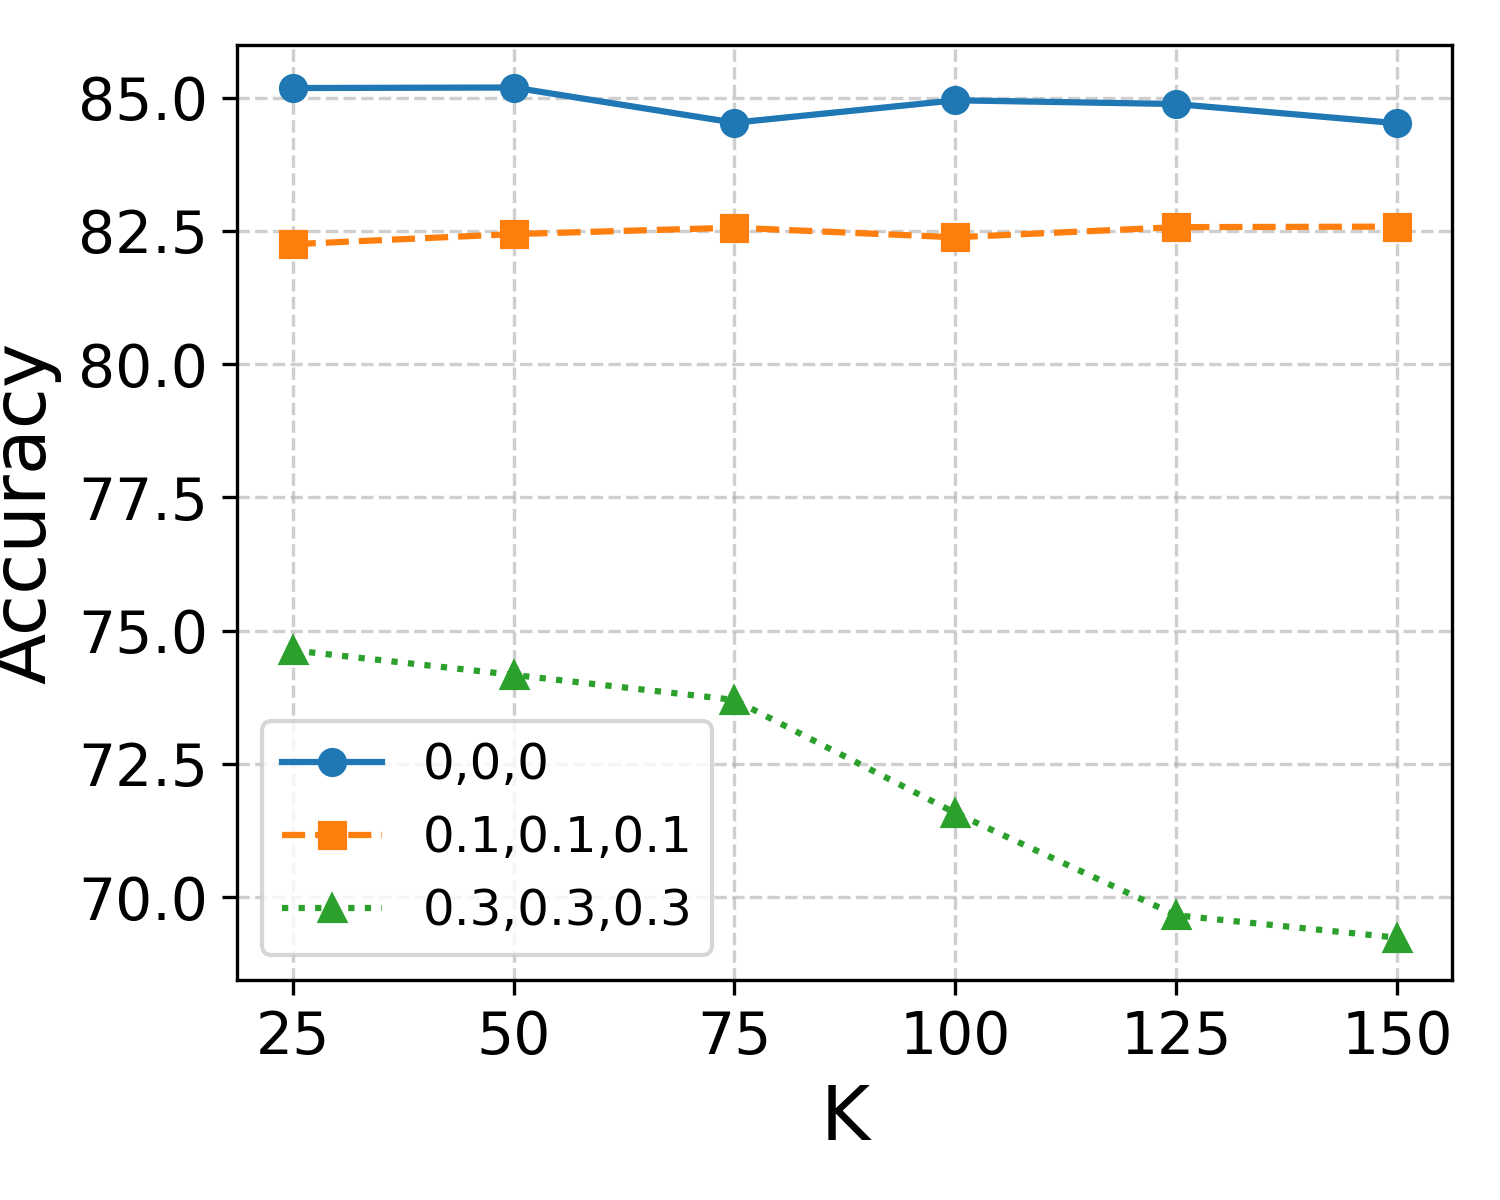
\includegraphics[width=\linewidth]{Figures/Cora_K_performance.png}
        \caption{Cora}
      \end{subfigure}
      \hfill 
      \begin{subfigure}[b]{0.23 \textwidth}
        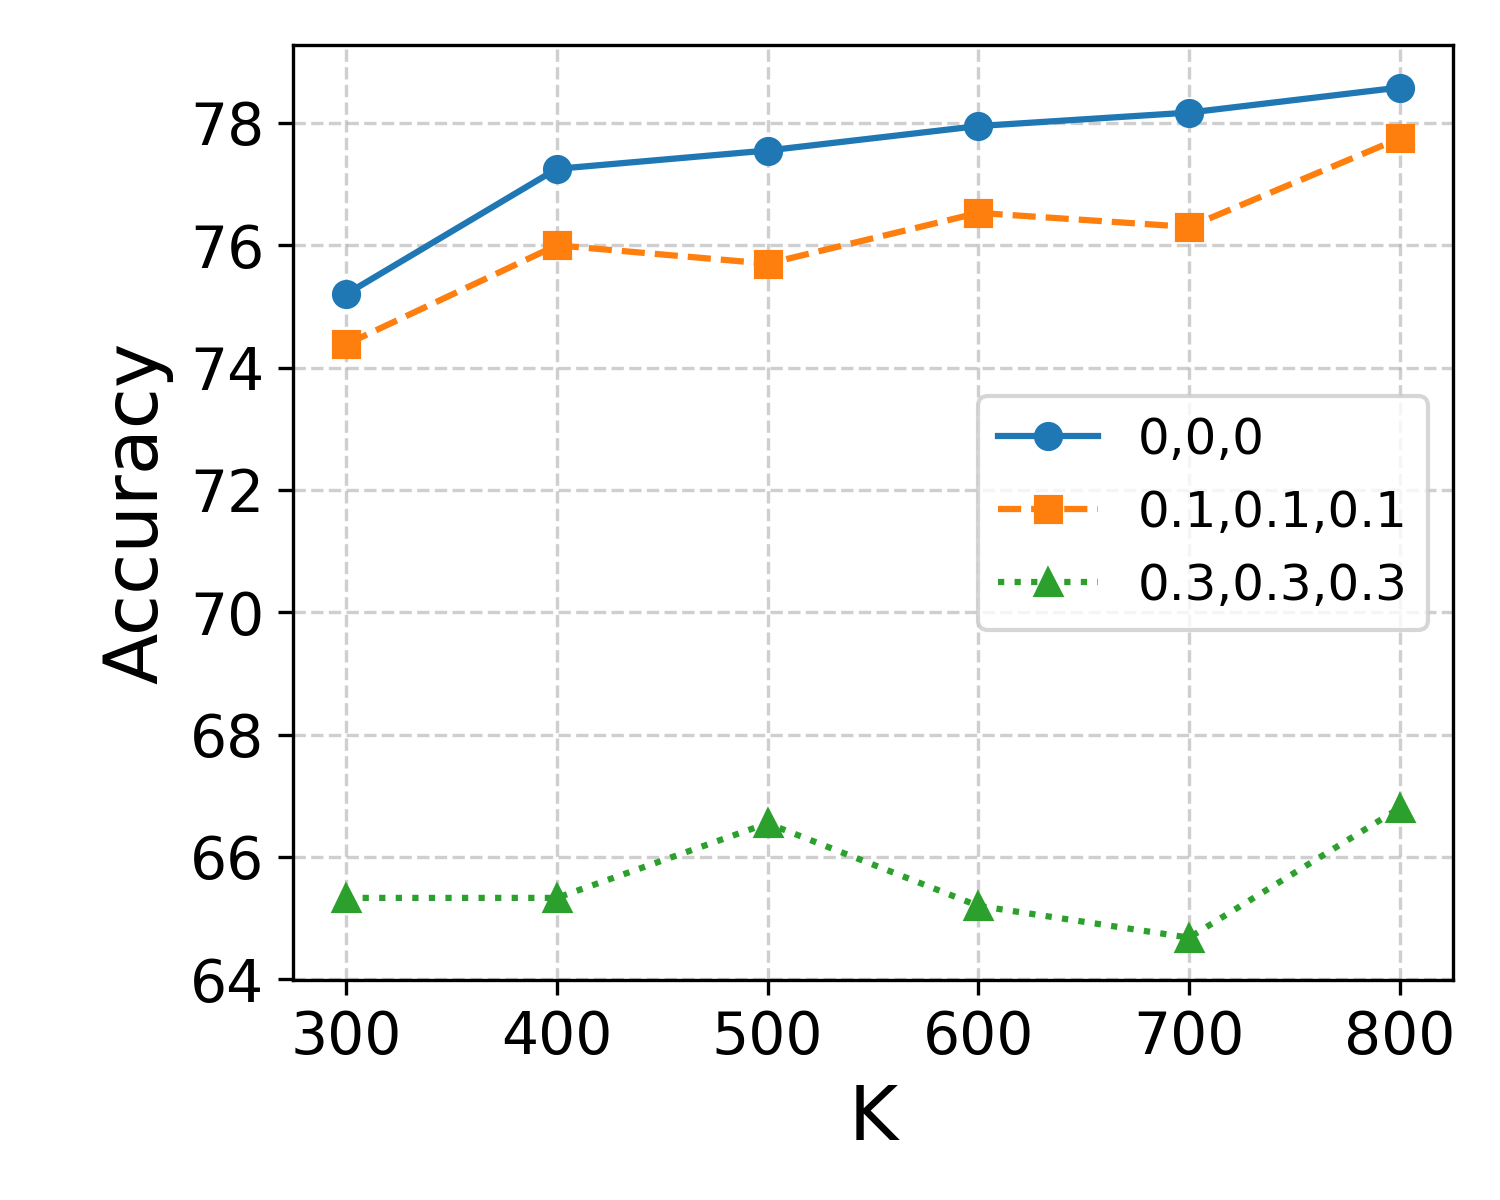
\includegraphics[width=\linewidth]{Figures/Pubmed_K_performance.png}
        \caption{Pubmed}
      \end{subfigure}
      \caption{The sensitivity of the hyper-parameter K,where the legend is the \{gr,lr,fr\}}
      \Description{Figure 4. Fully described in the text.}
      \label{fig:K_performance}
    \end{figure}

    \begin{figure}[htbp]
      \centering
      \begin{subfigure}[b]{0.23\textwidth}
        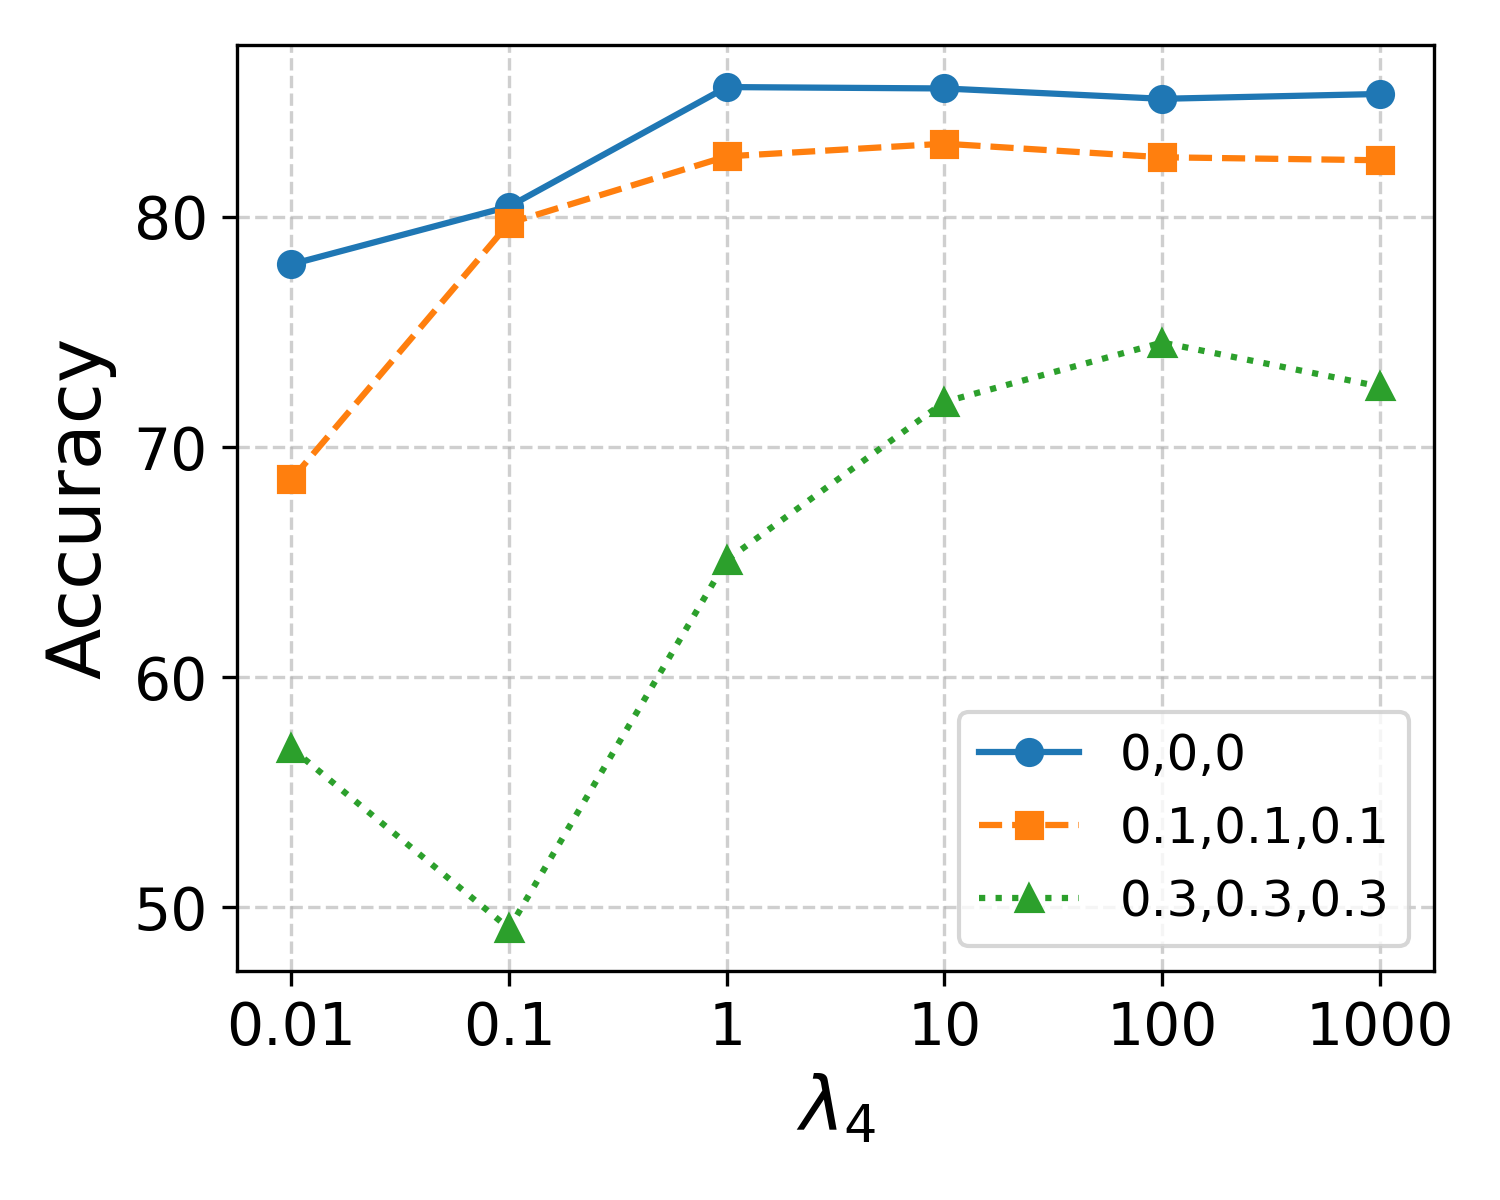
\includegraphics[width=\linewidth]{Figures/Cora_lambda_performance.png}
        \caption{Cora}
      \end{subfigure}
      \hfill 
      \begin{subfigure}[b]{0.23 \textwidth}
        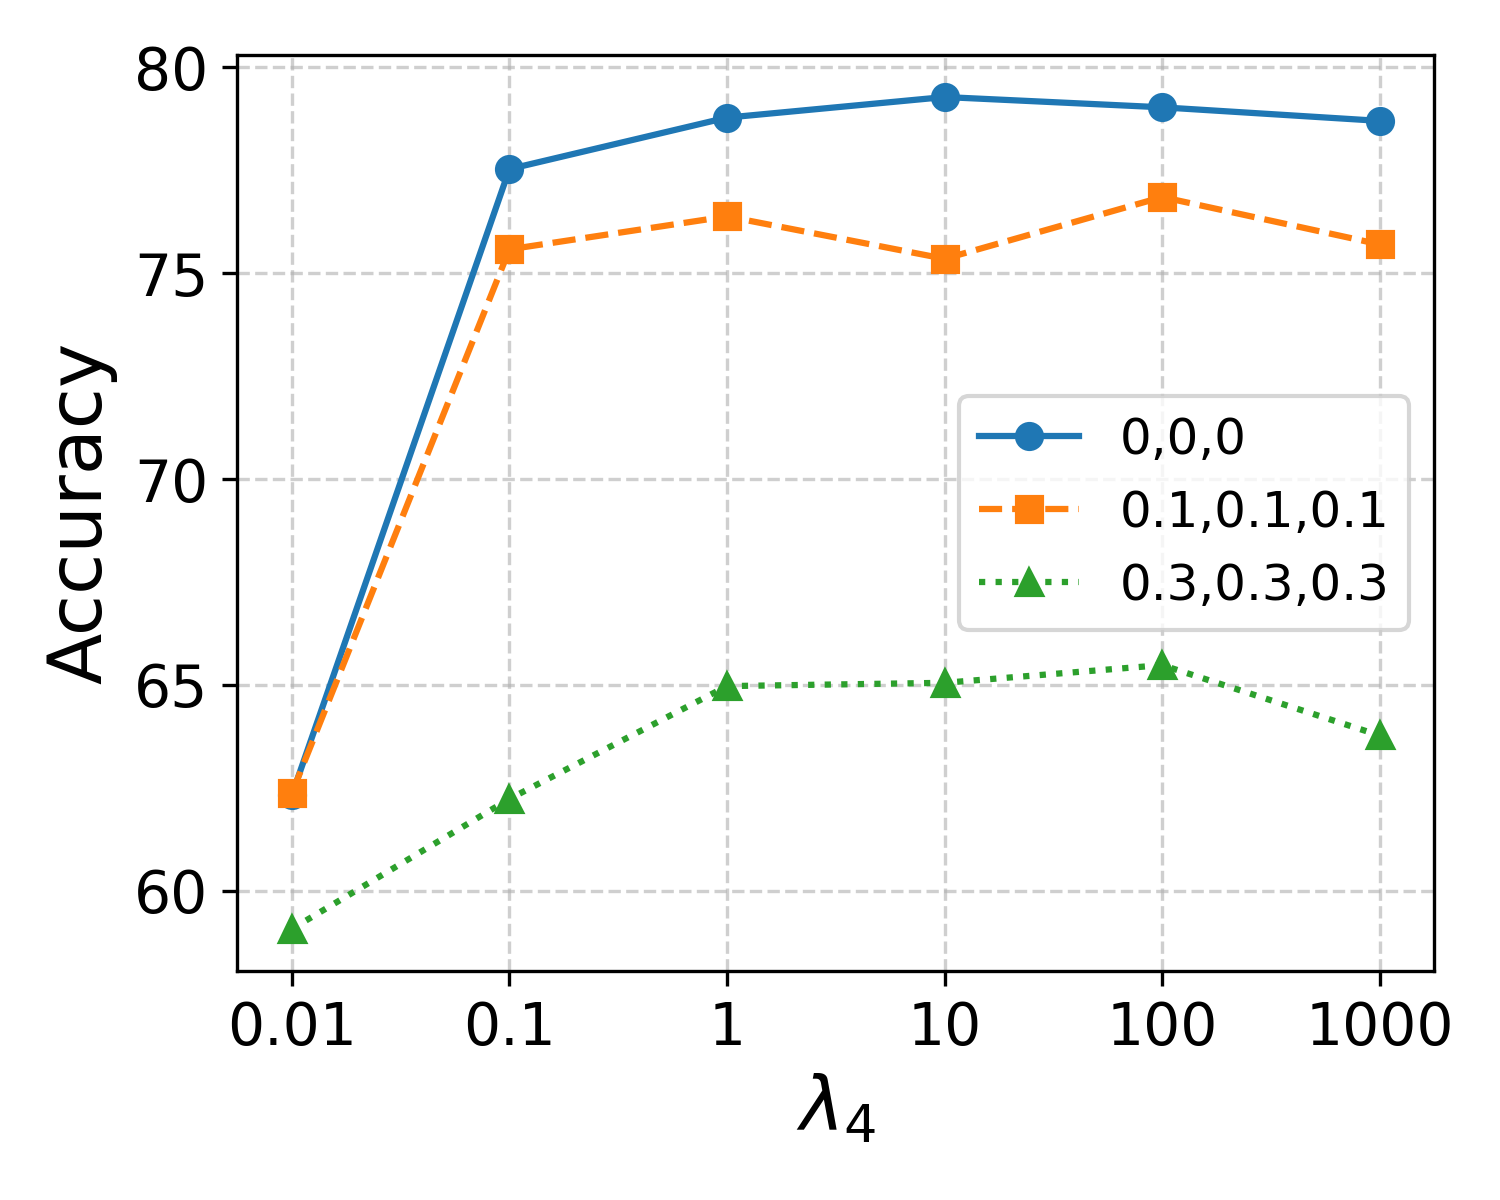
\includegraphics[width=\linewidth]{Figures/Pubmed_lambda_performance.png}
        \caption{Pubmed}
      \end{subfigure}
      \caption{The sensitivity of the hyper-parameter $\lambda_4$ ,where the legend is the \{gr,lr,fr\}}
      \Description{Figure 5. Fully described in the text.}
      \label{fig:lambda_performance}
    \end{figure}

    \begin{figure}[htbp]
      \centering
      \begin{subfigure}[b]{0.23\textwidth}
        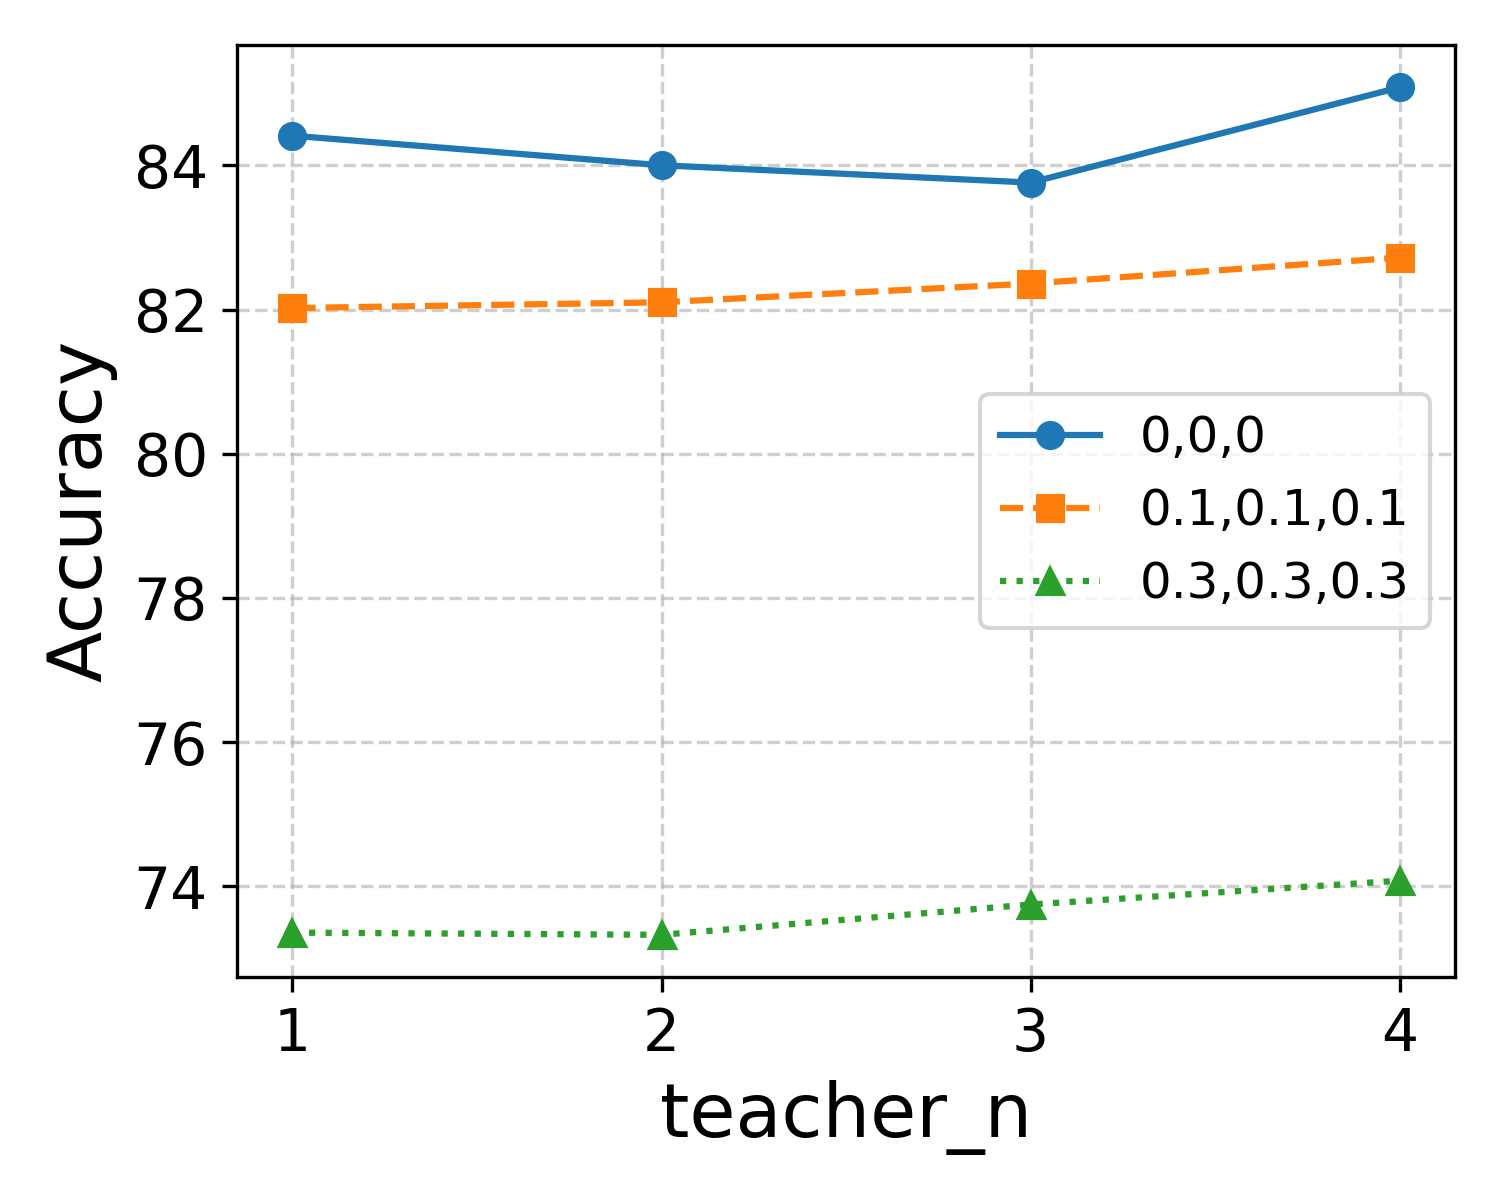
\includegraphics[width=\linewidth]{Figures/Cora_teacher_n_performance.png}
        \caption{Cora}
      \end{subfigure}
      \hfill 
      \begin{subfigure}[b]{0.23 \textwidth}
        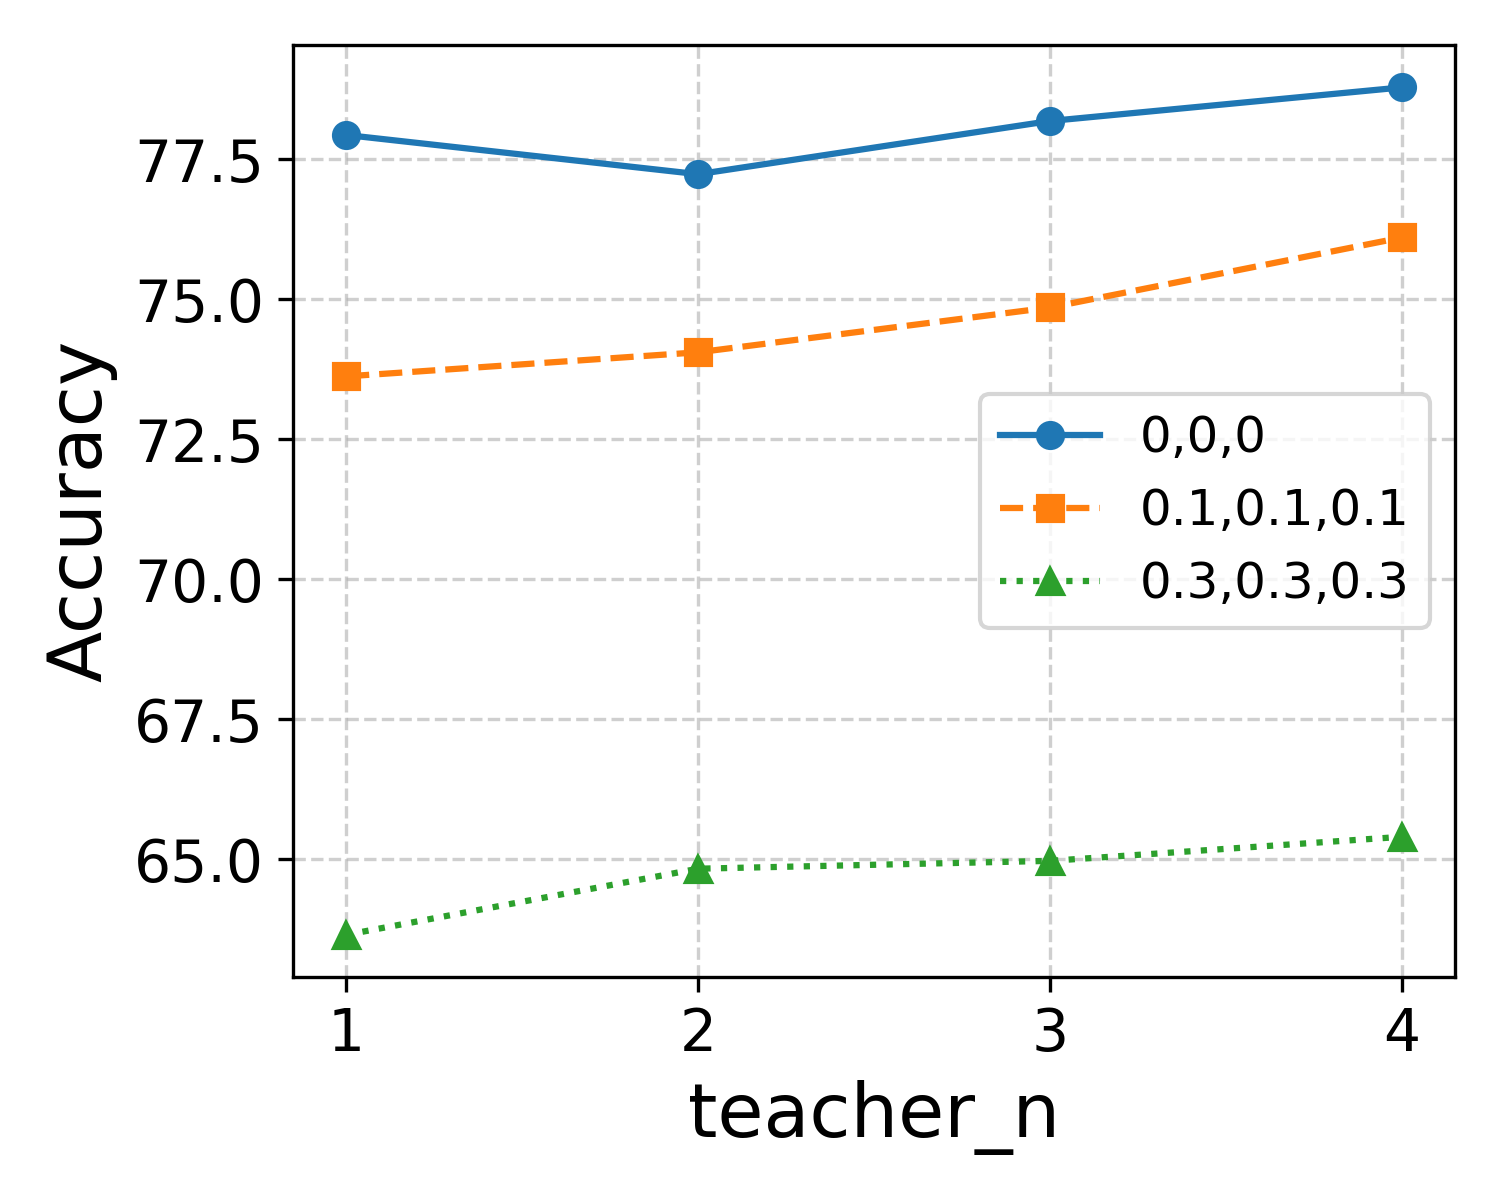
\includegraphics[width=\linewidth]{Figures/Pubmed_teacher_n_performance.png}
        \caption{Pubmed}
      \end{subfigure}
      \caption{The sensitivity of the hyper-parameter $teacher_n$, where the legend is the \{gr,lr,fr\}}
      \Description{Figure 6. Fully described in the text.}
      \label{fig:teacher_n_performance}
    \end{figure}
    
  \subsection{Efficiency Analysis (RQ4)}
    We conducted experiments to calculate the inference time for one sample on each dataset, using both the baseline method and TRINA.
    In Figure \ref{fig:intime}, we show the time to predict for one node in the baseline and TRINA for node classification tasks. From the figure, we can observe that GCN has the fastest inference speed. Next is Mid-GCN, but its inference speed on the Photo dataset is rather slow. The inference times of PRINGLE, RT-GNN and TRINA are similar, because their predictors all use weighted GCN. The model with the slowest inference speed is RNCGLN. Thus, it can be seen that the inference speed of our proposed model is acceptable.
    \begin{figure}[htbp]
      \centering
      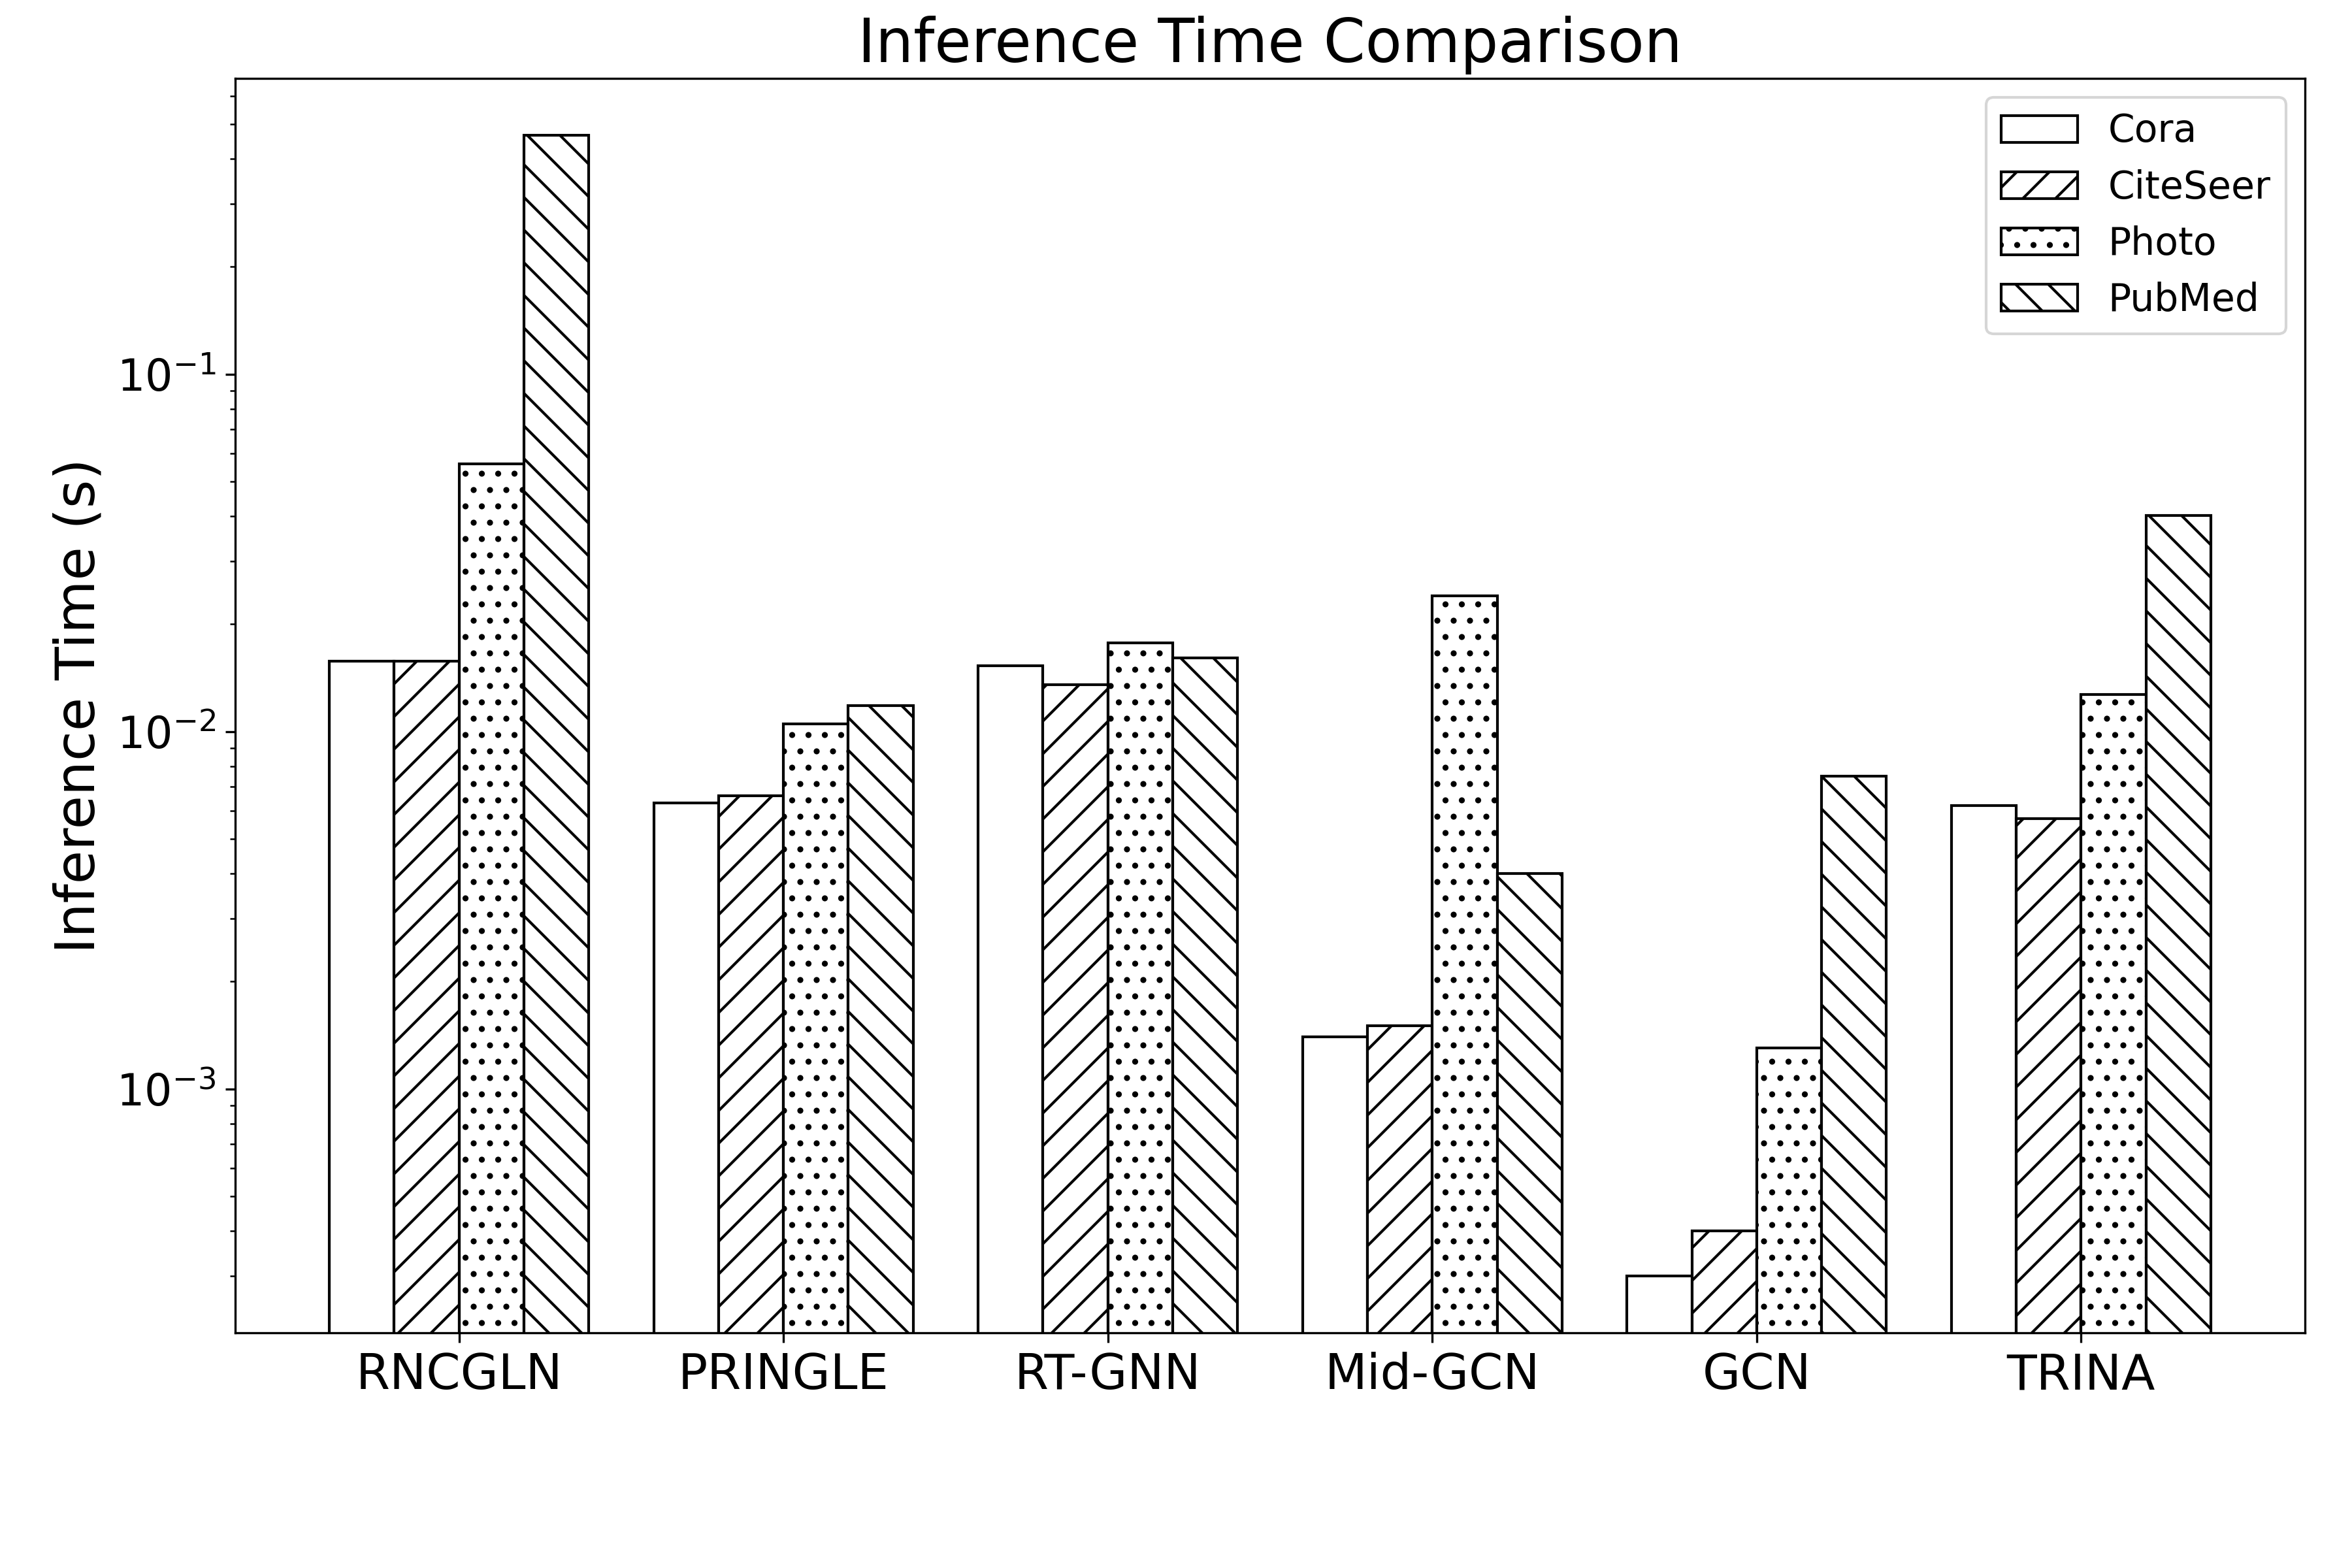
\includegraphics[width=.9\linewidth]{Figures/inference_time_comparison.png}
      \caption{Inference time (sec) comparison for a single node}
      \Description{Figure 7. Fully described in the text.}
      \label{fig:intime}
    \end{figure}
    
\section{Conclusion}
  We propose TRINA, a robust graph learning framework designed to address the challenging problem of trilateral noise in node features, graph structure, and labels. TRINA employs a two-stage learning strategy in which multiple teacher models generate reliable soft-label distributions and pseudo-labels to supervise a student model. This approach reduces the risk of error propagation commonly seen in previous methods. Furthermore, the SFC module iteratively refines both the graph topology and node features, enabling TRINA to adaptively suppress noise without assuming any part of the input is inherently clean. With Metis partitioning and adversarial subgraph embedding alignment, TRINA further scales to large graphs such as ogbn-arxiv while preserving robustness under trilateral noise. Extensive experiments on diverse datasets and noise types demonstrate that TRINA achieves SOTA performance and robustness. Ablation studies and efficiency analyses validate the effectiveness and practicality of each component.

%%
%% The acknowledgments section is defined using the "acks" environment
%% (and NOT an unnumbered section). This ensures the proper
%% identification of the section in the article metadata, and the
%% consistent spelling of the heading.
\begin{acks}
  This paper was supported by Beijing Institute of Technology No.xxxx.
\end{acks}


% \section*{Ethics and Privacy Statement}


%%
%% The next two lines define the bibliography style to be used, and
%% the bibliography file.
\bibliographystyle{ACM-Reference-Format}
\bibliography{reference_origin}


%%
%% If your work has an appendix, this is the place to put it.
\appendix

\begin{table*}
  \centering
  \caption{Accuracy w.r.t Different Noise Injection Methods}
  {\small
  \begin{tabular}{ccccccccc}
    \toprule
    Noise Type &Dataset&\{gr,lr,fr\} & RNCGLN &PRINGLE&RT-GNN&Mid-GCN&GCN&TRINA\\
    \midrule
    \multirow{12}{*}{Pair} & \multirow{3}{*}{Cora} &\{0,0,0\}&83.11±0.70&83.12±0.02&77.95±0.18&\underline{84.50±0.7}0&84.26±0.52&\textbf{85.35±0.35}\\
    &  &\{.1,.1,.1\}&74.05±1.90 &\underline{76.81±0.44}&71.88±1.54&76.37±0.18&75.07±0.68 & \textbf{82.38±0.19} \\
    &  &\{.3,.3,.3\}&\underline{61.72±1.79}&59.73±0.97&52.23±1.05&54.06±0.33&50.67±0.99&\textbf{70.89±0.86}\\
    & \multirow{3}{*}{CiteSeer} &\{0,0,0\}&70.63±1.11 &\underline{70.97±1.34}&67.55±1.93&70.55±0.45&67.98±0.62 &\textbf{72.35±0.32}  \\
    &  &\{.1,.1,.1\}&65.85±1.19&66.87±0.83&59.06±1.40&62.75±0.72&\textbf{68.40±1.42}&\textbf{68.08±0.86}\\
    &  &\{.3,.3,.3\}&49.43±0.86&\underline{53.53±2.42}&42.01±1.68&44.85±1.57&52.85±1.53&\textbf{55.05±1.63}\\
    & \multirow{3}{*}{Photo} &\{0,0,0\}&87.16±0.62&\textbf{94.16±0.15}&88.97±0.35&81.96±0.06&92.36±0.13&\textbf{93.98±0.15}\\
    &  &\{.1,.1,.1\}&78.81±0.74 &\underline{90.73±0.12}&85.65±0.35&74.10±0.49&88.58±0.32 & \textbf{91.14±0.89} \\
    &  &\{.3,.3,.3\}&58.52±1.47&\underline{81.27±0.18}&73.55±0.30&57.23±0.91&78.27±0.60&\textbf{84.47±0.42}\\
    & \multirow{3}{*}{Pubmed} &\{0,0,0\}&76.18±0.61 &75.30±0.37&\underline{78.21±1.30}&77.98±0.49&76.63±0.55 &\textbf{78.93±0.27}  \\
    &  &\{.1,.1,.1\}&69.10±0.65 &62.23±0.57&67.49±0.87&\underline{70.57±0.64}& 68.25±0.53& \textbf{74.25±0.34} \\
    &  &\{.3,.3,.3\}&56.90±1.44&49.47±1.52&48.34±5.10&\underline{62.32±0.81}&58.28±0.46&\textbf{63.25±0.34}\\
    \midrule
    
    \multirow{12}{*}{Feature Based} & \multirow{3}{*}{Cora} &\{0,0,0\}&83.11±0.70 &82.96±0.10&77.91±0.42&\underline{84.50±0.70}&84.26±0.52 &\textbf{85.47±0.11}  \\
    &  &\{.1,.1,.1\}&77.64±0.34 &78.52±0.14&76.43±0.92&\underline{81.45±0.95}&78.69±0.76 &\textbf{83.38±0.23}  \\
    &  &\{.3,.3,.3\}&65.11±1.56&\underline{66.00±0.73}&62.78±1.30&65.32±0.61&57.74±0.10&\textbf{75.54±0.37}\\
    & \multirow{3}{*}{CiteSeer} &\{0,0,0\}&70.63±1.11 &\underline{70.93±1.33}&67.59±1.72&70.55±0.45&67.98±0.62 & \textbf{72.25±0.18} \\
    &  &\{.1,.1,.1\}&68.78±0.31&\underline{69.23±0.60}&63.15±1.53&68.48±0.64&\underline{69.23±0.75}&\textbf{70.80±0.41}\\
    &  &\{.3,.3,.3\}&\underline{62.53±3.89}&60.97±0.69&47.56±2.67&56.65±0.70
    &60.18±2.03&\textbf{62.97±1.36}\\
    & \multirow{3}{*}{Photo} &\{0,0,0\}&87.16±0.62&\textbf{94.41±0.09}&89.07±0.44&81.97±0.07&92.36±0.13&\underline{93.89±0.15}\\
    &  &\{.1,.1,.1\}&76.77±0.88 &\textbf{91.78±0.21}&86.36±0.17&73.66±0.03&90.07±0.28 &\textbf{91.38±0.30}  \\
    &  &\{.3,.3,.3\}&57.62±2.64&\underline{86.35±0.32}&78.83±1.56&58.64±0.80&84.95±0.66&\textbf{87.90±0.49}\\
    & \multirow{3}{*}{Pubmed} &\{0,0,0\}&76.18±0.61&75.10±0.65&\textbf{78.25±1.24}&77.98±0.49&76.63±0.55&\textbf{78.95±0.09}\\
    &  &\{.1,.1,.1\}&66.73±2.16&62.77±0.09&66.61±1.56&69.70±1.53&\underline{70.18±0.33}&\textbf{70.85±0.57}\\
    &  &\{.3,.3,.3\}&\underline{53.53±2.29} &31.83±1.72&50.32±4.31&49.65±7.22& 49.88±1.03&\textbf{64.35±0.88}\\
    
    \midrule
    \multirow{12}{*}{Class Confusion} & \multirow{3}{*}{Cora} &\{0,0,0\}&83.11±0.70&83.10±0.04&77.77±0.22&\underline{84.50±0.70}&84.26±0.52&\textbf{85.48±0.12}\\
    &  &\{.1,.1,.1\}&70.15±0.62 &75.76±0.60&74.51±0.30&\underline{75.99±0.74}&74.91±0.46 &\textbf{79.39±0.21}  \\
    &  &\{.3,.3,.3\}&48.12±1.12&56.20±0.61&54.05±1.08&59.57±0.76&\underline{60.64±0.37}&\textbf{62.56±2.17}\\
    & \multirow{3}{*}{CiteSeer} &\{0,0,0\}&70.63±1.11 &\underline{70.93±1.33}&67.71±1.75&70.55±0.45&67.98±0.62 & \textbf{72.18±0.59} \\
    &  &\{.1,.1,.1\}&59.18±1.92&64.73±0.76&57.85±3.14&61.92±0.84&\underline{65.68±1.93}&\textbf{66.63±0.80}\\
    &  &\{.3,.3,.3\}&33.95±1.93 &45.50±0.75&39.99±1.22&42.62±1.32&\underline{48.93±1.92}& \textbf{53.75±0.79} \\
    & \multirow{3}{*}{Photo} &\{0,0,0\}&87.16±0.62&\textbf{94.30±0.08}&89.22±0.17&81.97±0.07&92.36±0.13&\underline{93.67±0.13}\\
    &  &\{.1,.1,.1\}&75.91±0.15 &\textbf{90.43±0.37}&85.88±0.38&72.69±0.02&89.10±0.40 & \underline{89.59±0.29} \\
    &  &\{.3,.3,.3\}&58.85±1.14&\textbf{80.16±0.39}&71.34±1.20&57.09±0.17&\textbf{80.23±0.21}&\textbf{78.70±1.47}\\
    & \multirow{3}{*}{Pubmed} &\{0,0,0\}&76.18±0.61&75.47±0.50&\underline{78.23±1.32}&77.98±0.49&76.63±0.55&\textbf{78.63±0.29}\\
    &  &\{.1,.1,.1\}&64.88±1.08&65.67±0.31&68.01±0.97&\textbf{69.90±0.76}&69.40±0.74&\textbf{69.58±0.44}\\
    &  &\{.3,.3,.3\}&42.50±1.90&41.87±2.60&\textbf{55.40±3.01}&\textbf{56.00±1.23}&53.48±0.90&46.85±0.63\\
    \bottomrule
  \end{tabular}}
  \label{tab:performence_dtn_app}
\end{table*}

\begin{table*}
  \centering
  \caption{Ablation Study}
  {\small
  \begin{tabular}{cccccccccc}
    \toprule
    \multirow{2}{*}{Noise Type} &\multirow{2}{*}{Dataset}&\multirow{2}{*}{\{gr,lr,fr\}}
    & TRINA\_T & TRINA\_T & TRINA\_T & TRINA\_T &\multirow{2}{*}{TRINA\_T}  &\multirow{2}{*}{TRINA}\\
    &&& w/ CE & w/o SC & w/o FC & w/ $X_o$ & &\\
    \midrule
    \multirow{6}{*}{Uniform} & \multirow{3}{*}{Cora} &\{0,0,0\}&82.87±0.29 &79.28±0.27&83.28±0.50 &\underline{83.32±0.37}&83.16±0.44& \textbf{85.19±0.86} \\
    &  &\{.1,.1,.1\}&81.26±0.46 &71.76±0.77&79.54±0.57 &80.72±0.36&\textbf{81.60±0.30}&\underline{81.33±0.32}  \\
    &  &\{.3,.3,.3\}&72.84±1.40 &60.93±0.69&67.32±0.56 &71.71±0.80&\textbf{73.51±0.37}&\underline{73.18±1.00 } \\
    & \multirow{3}{*}{Pubmed} &\{0,0,0\}&77.20±0.64 &70.32±1.61& 77.40±0.92&77.83±0.65&\underline{78.12±0.85}&\textbf{78.78±0.43}  \\
    &  &\{.1,.1,.1\}&72.43±1.46 &65.22±1.47& 70.38±2.56&71.38±0.96&\underline{73.55±0.63}&\textbf{76.10±0.24}  \\
    &  &\{.3,.3,.3\}&62.52±1.04&53.73±1.03& 57.80±1.69&59.57±2.56&\underline{63.45±1.65}&\textbf{65.40±0.51}  \\
    \midrule
    \multirow{6}{*}{Pair} & \multirow{3}{*}{Cora} &\{0,0,0\}&83.10±0.30 &79.28±0.27&83.19±0.59 &83.38±0.44&\underline{83.45±0.44}&\textbf{85.35±0.35}  \\
    &  &\{.1,.1,.1\}&79.82±1.30 &71.48±1.67&78.89±0.54 &79.92±1.71&\underline{80.52±1.34}&\textbf{82.38±0.19}  \\
    &  &\{.3,.3,.3\}&68.47±0.97 &55.12±0.79&63.69±1.39 &68.40±1.11&\underline{70.03±1.39}&\textbf{70.89±0.86 } \\
    & \multirow{3}{*}{Pubmed} &\{0,0,0\}&77.20±0.70&70.32±1.61&\underline{77.60±0.67} &77.53±0.75&77.75±0.54&\textbf{78.93±0.27}  \\
    &  &\{.1,.1,.1\}&68.90±1.14 &62.95±1.27&70.50±0.76 &70.62±0.84&\underline{70.80±1.86}&\textbf{74.25±0.34}  \\
    &  &\{.3,.3,.3\}&58.40±1.38 &56.48±1.11& 56.08±1.68&57.15±1.39&\underline{61.73±1.61}&\textbf{63.25±0.34}  \\
    \midrule
    \multirow{6}{*}{Feature Based} & \multirow{3}{*}{Cora} &\{0,0,0\}&82.74±0.36 &79.28±0.27&83.15±0.32 &83.19±0.35&\underline{83.29±0.56}&\textbf{85.47±0.11}  \\
    &  &\{.1,.1,.1\}&81.46±0.54 &74.99±0.39&80.07±0.62 &81.76±0.30&\underline{82.33±0.15}&\textbf{83.38±0.23}  \\
    &  &\{.3,.3,.3\}&73.24±1.54 &66.01±1.07&67.42±0.67 &71.20±1.06&\underline{73.26±0.42}&\textbf{75.54±0.37}  \\
    & \multirow{3}{*}{Pubmed} &\{0,0,0\}&77.42±0.68 &70.32±1.61& \underline{77.73±0.69}&77.68±0.66&77.62±1.01&\textbf{78.95±0.09 } \\
    &  &\{.1,.1,.1\}& 67.38±1.50&65.22±1.65& 66.80±1.61&65.30±2.13&\underline{67.72±2.27}&\textbf{70.85±0.57}  \\
    &  &\{.3,.3,.3\}&59.58±1.37 &54.80±1.95& 54.43±3.94&59.85±5.21&\underline{60.23±1.67}&\textbf{64.35±0.88}  \\
    \midrule
    \multirow{6}{*}{Class Confusion} & \multirow{3}{*}{Cora} &\{0,0,0\}&82.44±0.56 &79.28±0.27&83.00±0.30 &83.07±0.49&\underline{83.25±0.62}&\textbf{85.48±0.12}  \\
    &  &\{.1,.1,.1\}&\underline{77.49±0.74} &68.85±2.07&77.24±0.70 &76.67±1.07&75.92±0.91&\textbf{79.39±0.21}  \\
    &  &\{.3,.3,.3\}&\textbf{66.24±0.80} &60.83±1.10&56.91±2.51 &61.80±1.28&\underline{65.15±0.43}&62.56±2.17  \\
    & \multirow{3}{*}{Pubmed} &\{0,0,0\}&77.05±0.79 &70.32±1.61&\underline{77.70±0.60} &77.47±0.92&77.68±0.60&\textbf{78.63±0.29}  \\
    &  &\{.1,.1,.1\}&67.68±2.23 &\textbf{70.32±1.61}& 67.48±0.31&67.90±0.27&68.42±1.38&\underline{69.58±0.44}  \\
    &  &\{.3,.3,.3\}&\textbf{47.52±3.31} &44.53±2.86&39.43±1.22 &42.30±1.05&43.32±0.79&\underline{46.85±0.63}  \\
    \bottomrule
  \end{tabular}}
  \label{tab:ablation_app}
\end{table*}

\section{Additional Experiments}
  \subsection{Baselines}
    \begin{itemize}
        \item GCN~\cite{kipf2016semi}: GCN is a popular graph convolutional network based on spectral theory.
        \item RNCGLN ~\cite{zhu2024robust}: This method utilizes multi-hop graph and pseudo labels to separately handle graph structure noise and label noise.
        \item PRINGLE ~\cite{in2024noise}:This method proposes the noise hypothesis FDGN, which believes that both the noise in the graph structure and the noise in the labels originate from feature noise. And based on this causal relationship, it handles the trilateral noise.
        \item RTGNN ~\cite{qian2023robust}:This method utilizes an edge classifier for graph augmentation, and uses the loss and confidence of labeled and unlabeled points to separately select clean samples and assign pseudo labels.
        \item Mid-GCN~\cite{huang2023robust}:This method utilizes mid-frequency signals on graphs to filter out noisy graph structure noise.
    \end{itemize}


  \subsection{Accuracy w.r.t Different Noise Injection Methods}
    Here, we present a comparison of the model performance under various noise ratios.The average performance and standard deviation over four independent runs are reported in Table~\ref{tab:performence_dtn_app}. From the results, we make the following observations:
    (1) As the noise becomes increasingly severe, the performance of various methods also deteriorates more significantly. However, on all the noise ratios, TRINA achieved the best performance in almost every case.
    (2) Even at a high noise ratio, TRINA can still maintain relatively stable robustness, typically experiencing less performance degradation compared to other models.
    (3) Under the noise type of class confusion, the performance of each model declined the most, but TRINA still achieved relatively excellent results. However, on the Pubmed dataset, when the noise level was high, all models were subjected to very significant perturbation.

  \subsection{Ablation Study}
    To evaluate the effectiveness of each component in TRINA, we conduct an ablation study based on its single-teacher variant, denoted as ``TRINA\_T''.  Specifically, we assess the contribution of the GCE loss by replacing it with standard cross-entropy, resulting in the variant ``TRINA\_T w/ CE''. We also evaluate the impact of the structure cleaning (SC) and feature cleaning (FC) modules by removing them individually, referred to as``TRINA\_T w/o SC'' and  ``TRINA\_T w/o FC'', respectively.  In addition, we test the role of iterative feature refinement in structure cleaning by replacing the updated feature $X_t^1$ in Eq.~\ref{eq:rep} with the original noisy feature $X_o$, denoted as ``TRINA\_T w/ $X_o$''.
    Detailed results under varying noise rates are provided in Table~\ref{tab:ablation_app}. From the results, we draw the following observations:
    (1) Under both pair noise and feature-based noise, under various levels of noise, each module of the model achieved the most significant results.
    (2) Under uniform noise, in most cases, each part of the model plays an important role, especially the SC, FC modules, and the use of $X_t$.
    (3) Under the Class confusion noise, at each noise ratio, each module of the model played a certain role.


\end{document}
\endinput
%%
%% End of file `sigconf.tex'.
